\documentclass[12pt,AutoFakeBold]{article} 

\usepackage[数字信号处理]{XDULabreport}  % 载入 XDULabreport 模板文件,[]中填写科目名称,科目名称,默认为电子线路实验(I)
\problem{IIR 数字滤波器设计及结构}  % 请在此处填写问题内容
\labdate{2021年12月06日} % 实验日期
% 其他参数在宏包中进行更改,其中学院,班级,姓名,学号均在sty宏包内进行更改
% \usepackage{fourier}  % 这是 fourier 字体,更柔和 

\newfontfamily\digi{DigifaceWide Regular} % 将数码管字体引入

%% 如果你需要中文的一级标题编号,如“一、”、“二、”等,请把下面两行取消注释
% \RequirePackage{zhnumber} % change section number to chinese
% \titleformat{\section}{\Large\bfseries\rmfamily}{\zhnum{section}、}{0em}{}

% 文档开始
        
\begin{document}

\maketitle
\setcounter{tocdepth}{2}
\tableofcontents  % 生成目录

% 正文标题
\makeatletter
\begin{center}
    \LARGE \textbf{\textsf{\@problem}}
\end{center}
\makeatother

\section{实验目的}

设计计算机程序,根据滤波器的主要技术指标设计 IIR 数字巴特沃斯和切比雪夫低通、高通、带通和带阻滤波器;绘制滤波器的幅频特性和相频特性曲线,验证滤波器的设计结果是否达到设计指标要求;画出数字滤波器的直接型、级联型、并联型结构信号流图。

\section{实验原理}

\subsection{模拟低通滤波器的技术指标}

模拟低通滤波器的技术指标有 $\alpha_p$,$\Omega_p$,$\alpha_s$,$\Omega_s$,其中 $\Omega_p$ 和 $\Omega_s$ 分别称为通带截至频率和阻带截止频率,$\alpha_p$ 是通带 ($0\le\Omega\le\Omega_p$) 内的最大允许衰减,$\alpha_s$ 是阻带 ($\Omega\ge\Omega_p$) 内的最小允许衰减。$\alpha_p$ 和 $\alpha_s$ 一般用分贝 (dB) 表示,对于单调下降的幅频响应,$\alpha_p$ 和 $\alpha_s$ 可分别表示为
%
\begin{equation} \label{eq:1}
\alpha_p=10\lg\frac{|H_a(j0)|^2}{|H_a(j\Omega_p)|^2}\mathrm{dB}
\end{equation}
%
和
%
\begin{equation} \label{eq:2}
\alpha_s=10\lg\frac{|H_a(j0)|^2}{|H_a(j\Omega_s)|^2}\mathrm{dB}
\end{equation}
%

如果 $\Omega=0$ 处的 $|H_a(j0)|=1$,即为幅度归一化的模拟滤波器,此时 $\alpha_p$ 和 $\alpha_s$ 可表示为
%
\begin{equation}
\alpha_p=-10\lg|H_a(j\Omega_p)|^2\mathrm{dB}
\end{equation}
%
和
%
\begin{equation}
\alpha_s=-10\lg|H_a(j\Omega_s)|^2\mathrm{dB}
\end{equation}
%

当 $|H_a(j\Omega_c)|=\frac{\sqrt{2}}{2}$ 时,$-10\lg|H_a(j\Omega_c)|^2=3\mathrm{dB}$,故称 $\Omega_c$ 为模拟低通滤波器的 $3dB$ 截止频率。

\subsection{巴特沃斯模拟低通滤波器设计步骤}

\begin{enumerate}[1.]
\item 根据模拟滤波器的设计指标 $\Omega_p$, $\Omega_s$, $\alpha_p$, $\alpha_s$,确定滤波器的阶数N
\begin{equation}
N=\frac{\lg[(10^{0.1\alpha_p}-1)/(10^{0.1\alpha_s}-1)]}{2\lg(\Omega_p/\Omega_s)}
\end{equation}
取 $N$ 为比计算结果大的最小整数,就是巴特沃斯模拟低通滤波器的阶数。

\item 确定滤波器的 $3\mathrm{dB}$ 截止频率
\begin{equation}
\Omega_{cp}=\frac{\Omega_p}{\sqrt[2N]{10^{0.1\alpha_p}-1}},\quad
\Omega_{cs}=\frac{\Omega_s}{\sqrt[2N]{10^{0.1\alpha_s}-1}}
\end{equation}
实际设计时,$\Omega_c$ 可在 $\Omega_{cp}\le\Omega_c\le\Omega_{cs}$ 范围内选择。

\item 按照 $p_k=\displaystyle\Omega_ce^{j\pi\left(\frac{2k+N-1}{2N}\right)}\ (k=1,2,\cdots,N)$ 求出 $N$ 个极点,将极点代入代入 (\ref{Hs}) 式得到滤波器的系统函数 $H_a(s)$。
\begin{equation}
H_a(s)=\frac{\Omega_c^N}{\displaystyle\prod_{k=1}^N(s-p_k)} \label{Hs}
\end{equation}
\end{enumerate}

\subsection{切比雪夫 I 型低通滤波器设计步骤}

\begin{enumerate}[1.]
\item 确定模拟滤波器的设计指标 $\Omega_p$, $\Omega_s$, $\alpha_p$, $\alpha_s$ 等

\item 确定参数 $\epsilon$
\begin{equation}
\epsilon=\sqrt{10^{0.1\alpha_p}-1}
\end{equation}

\item 确定滤波器的阶数 $N$,取 $N$ 为比计算结果大的最小整数,就是切比雪夫模拟低通滤波器的阶数
\begin{equation}
N=\mathrm{arccosh}\left(\frac{10^{0.1\alpha_s}-1}{10^{0.1\alpha_p}-1}\right)^{\frac{1}{2}}/\mathrm{arccosh}(\Omega_s/\Omega_p)
\end{equation}

\item 由 (\ref{pole}) 式和 (\ref{para}) 式求归一化切比雪夫 I 型低通滤波器的极点 $p_{nk}(k=1,2,3,\cdots,N)$
\begin{align} \label{pole}
p_{nk}=\sigma_k+j\Omega_k,\quad k=1,2,\cdots,N
\end{align}
%
\begin{subequations}
\label{para}
\begin{align}
\sigma_k&=-\sinh(\beta)\sin\frac{(2k-1)\pi}{2N} \\
\Omega_k&=-\cosh(\beta)\cos\frac{(2k-1)\pi}{2N} \\
\beta&=\frac{\mathrm{arcsinh}(1/\sigma)}{N} 
\end{align}
\end{subequations}

\item 由 (\ref{even}) 式(N 为偶数)或 \ref{odd} 式(N 为奇数) 获得归一化 CB I 型低通滤波器的系统函数 $H_n(s)$。
\begin{equation}
H_n(s)=\frac{1}{\sqrt{1+\epsilon^2}}\prod_{k=1}^{N/2}\frac{(\sigma_k^2+\Omega_k^2)}{s^2-2\sigma_ks+(\sigma_k^2+\Omega_k^2)} \label{even}
\end{equation}
%
\begin{equation}
H_n(s)=\frac{\sinh\beta}{1+\sinh\beta}\prod_{k=1}^{N/2}\frac{(\sigma_k^2+\Omega_k^2)}{s^2-2\sigma_ks+(\sigma_k^2+\Omega_k^2)} \label{odd}
\end{equation}

\item 去归一化的切比雪夫 I 型低通滤波器的系统函数为
\begin{equation}
H_a(s)=H_n(s/\Omega_p)
\end{equation}
\end{enumerate}

\subsection{切比雪夫 II 型低通滤波器设计步骤}

\begin{enumerate}[1.]
\item 确定模拟滤波器的设计指标 $\Omega_p$, $\Omega_s$, $\alpha_p$, $\alpha_s$ 等

\item 由阻带衰减 $\alpha_s$ 确定滤波器参数 $\epsilon$
\begin{equation}
\epsilon=\frac{1}{\sqrt{10^{0.1\alpha_p}-1}}
\end{equation}

\item 由通带衰减确定滤波器阶数 $N$,取 N 为比结果大的最小整数,就是切比雪夫模拟低通滤波器的阶数
\begin{equation}
N=\mathrm{arccosh}\left(\frac{1}{\epsilon\sqrt{10^{0.1\alpha_p}-1}}\right)/\mathrm{arccosh}(\Omega_s/\Omega_p)
\end{equation}

\item 由 \ref{polezero} 式求归一化切比雪夫 II 型低通滤波器的极点 $q_{nk}$ 和零点 $z_{nk}$
\begin{subequations}
\label{polezero}
\begin{align}
q_{nk}&=\frac{1}{p_{nk}},\quad k=1,2,\cdots,N \\
z_{nk}&=\frac{1}{\cos\left(\frac{(2k-1)\pi}{2N}\right)},\quad k=1,2,\cdots,N
\end{align}
\end{subequations}

\item 由 (\ref{even2}) 式(N 为偶数)或 \ref{odd2} 式(N 为奇数) 获得归一化 CB II 型低通滤波器的系统函数 $H_n(s)$。
\begin{equation}
H_n(s)=\prod_{k=1}^{N/2}\frac{(|q_{nk}|^2/|z_{nk}|^2)(s^2+|z_{nk}|^2)}{(s^2-2\mathrm{Re}[q_{nk}]s+|q_{nk}|^2)} \label{even2}
\end{equation}
%
\begin{equation}
H_n(s)=\frac{1/\sinh\beta}{s+1/\sinh\beta}\prod_{k=1}^{(N-1)/2}\frac{(|q_{nk}|^2/|z_{nk}|^2)(s^2+|z_{nk}|^2)}{(s^2-2\mathrm{Re}[q_{nk}]s+|q_{nk}|^2)} \label{odd2}
\end{equation}

\item 去归一化的切比雪夫 I 型低通滤波器的系统函数为
\begin{equation}
H_a(s)=H_n(s/\Omega_s)
\end{equation}
\end{enumerate}


\section{实验过程}

\subsection{巴特沃斯滤波器设计} \label{sec:p1}

MATLAB 信号处理工具箱中提供了设计巴特沃斯模拟滤波器函数 buttord、buttap 和 butter:
%
\begin{enumerate}[(1)]
\item \lstinline[language=Matlab]|[N,Wc]=buttord(Wp,Ws,Rp,Rs,'s')|

用于计算巴特沃斯模拟低通滤波器的阶 N 和 3dB 截至频率 Wc。其中,Wp 和 Ws 是分别是滤波器的通带截至频率 $\Omega_p$ 和阻带截止频率 $\Omega_s$,单位为 rad/s;Rp 和 Rs 分别是通带最大衰减系数 $\alpha_p$ 和阻带最小衰减系数 $\alpha_s$,单位为 dB。

\item  \lstinline[language=Matlab]|[z,p,G]=buttap(N)|
用于计算 N 阶巴特沃斯归一化 ($\Omega_c=1$) 模拟低通滤波器系统函数的零、极点和增益因子,返回长度为 $N$ 的向量 z 和 p 分别给出 N 个零点和极点,$G$ 是滤波器增益。得到的滤波器系统函数形式为:
%
\begin{equation}
H_a(s)=\frac{Q_a(s)}{P_a(s)}=G\frac{(s-z_1)(s-z_2)\cdots(s-z_N)}{(s-p_1)(s-p_2)\cdots(s-p_N)}
\end{equation}
%
其中,$z_k$ 和 $p_k$ 分别是向量 z 和 p 的第 k 个元素。

\item \lstinline[language=Matlab]|[B,A]=butter(N,Wc,'ftype','s')|
用于计算巴特沃斯模拟滤波器系统函数中分子和分母多项式系数向量 B 和 A。ftype 缺省时,设计低通滤波器;ftype=high 时,设计高通滤波器;ftype=stop 时,设计带阻滤波器,此时 Wc 为向量 [Wcl, Wcu],Wcl 和 Wcu 分别是带阻滤波器的通带 3dB 下、上截止频率;Wc 为向量 [Wcl, Wcu],且 ftype 缺省时,设计带通滤波器,带通的频率区间为 Wcl<$\Omega$<Wcu。s 缺省时,设计数字滤波器。
\end{enumerate}

\subsubsection{低通}

设置参数通带截止频率 Wp=0.2,阻带截止频率 Ws=0.4,通带最大衰减系数 Rp=1,阻带最小衰减系数 Rs=10。数字巴特沃斯低通滤波器频率响应曲线如图 \ref{fig:LPBF} 所示。$\omega=0.2$ 时幅度为 -0.3dB,$\omega=0.4$ 时幅度为 -10.1dB,通带满足指标要求,阻带满足指标要求,过渡带比指标要求的窄。

\begin{figure}[hbtp]
	\centering
	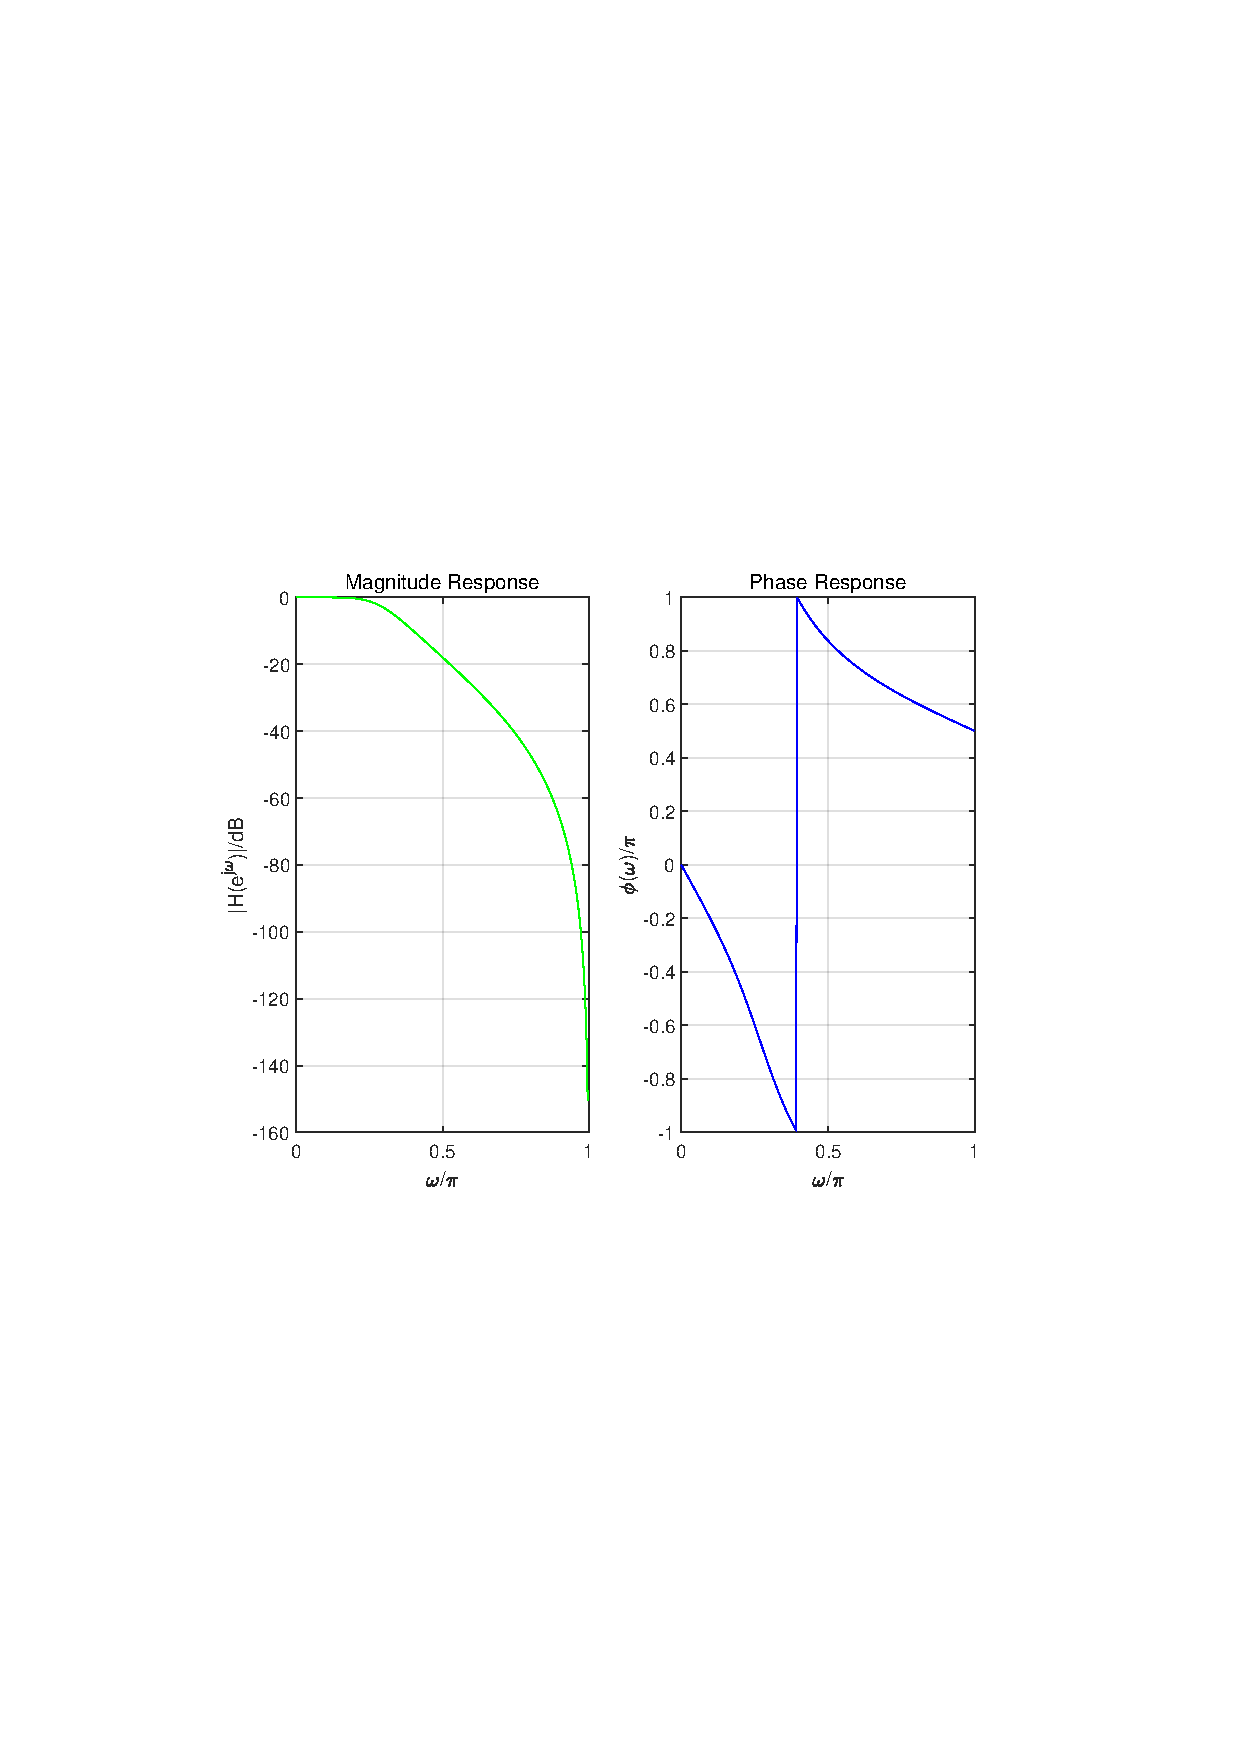
\includegraphics[width=14cm]{figure/LPBF.pdf}
	\caption{数字巴特沃斯低通滤波器频率响应曲线} \label{fig:LPBF}
\end{figure}


\subsubsection{高通}

设置参数通带截止频率 Wp=0.4,阻带截止频率 Ws=0.2,通带最大衰减系数 Rp=1,阻带最小衰减系数 Rs=10。数字巴特沃斯高通滤波器频率响应曲线如图 \ref{fig:HPBF} 所示。$\omega=0.2$ 时幅度为 -10.0dB,$\omega=0.4$ 时幅度为 -0.3dB,通带满足指标要求,阻带满足指标要求,过渡带比指标要求的窄。

\begin{figure}[hbtp]
	\centering
	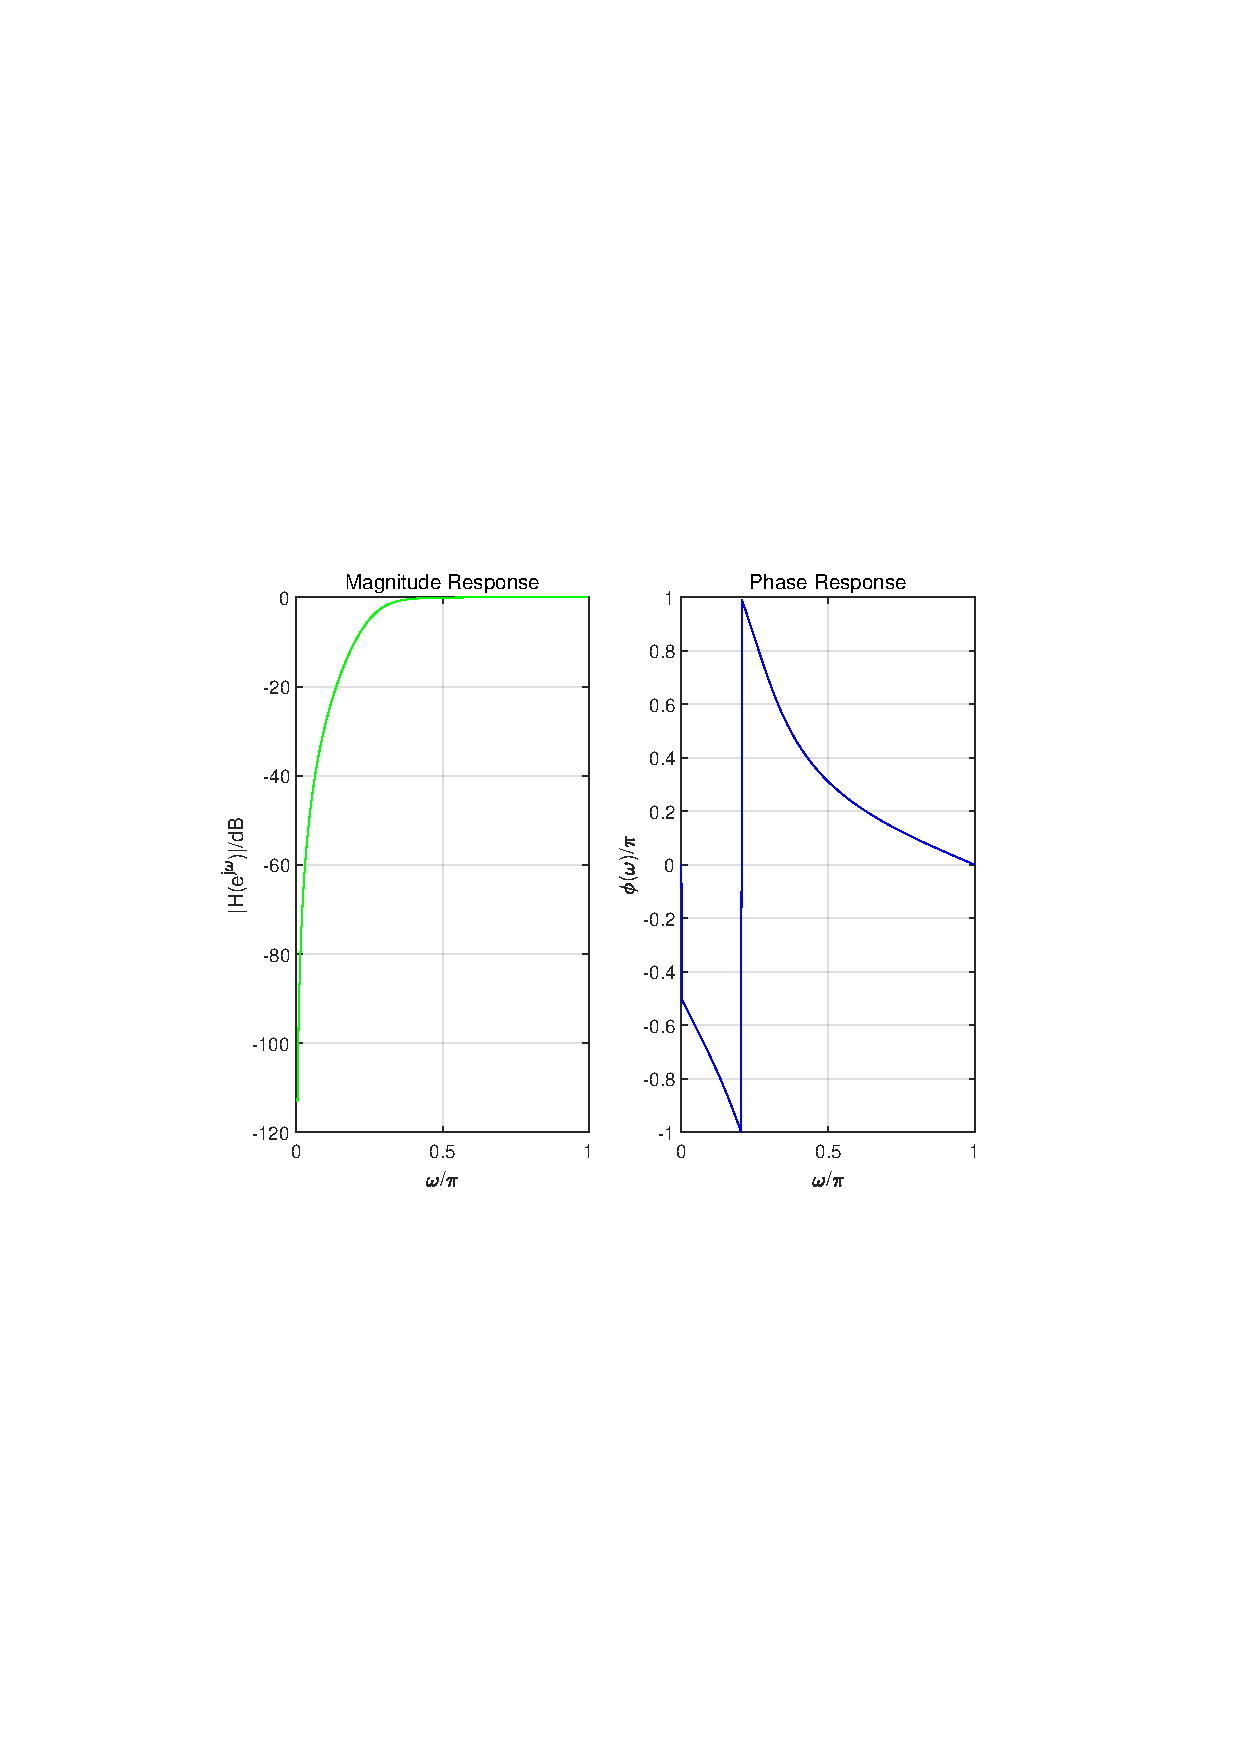
\includegraphics[width=14cm]{figure/HPBF.pdf}
	\caption{数字巴特沃斯高通滤波器频率响应曲线} \label{fig:HPBF}
\end{figure}


\subsubsection{带通}

设置参数通带截止频率 Wp=[0.2,0.4],阻带截止频率 Ws=[0.1,0.5],通带最大衰减系数 Rp=1,阻带最小衰减系数 Rs=10。数字巴特沃斯带通滤波器频率响应曲线如图 \ref{fig:BPBF} 所示。设置参数通带截止频率 Wp=0.4,阻带截止频率 Ws=0.2,通带最大衰减系数 Rp=1,阻带最小衰减系数 Rs=10。数字巴特沃斯高通滤波器频率响应曲线如图 \ref{fig:HPBF} 所示。$\omega=0.2$ 时幅度为 -0.4dB,$\omega=0.4$ 时幅度为 -1.0dB,$\omega=0.1$ 时幅度为 -23.5dB,$\omega=0.5$ 时幅度为 -10.4dB,通带满足指标要求,阻带满足指标要求,过渡带比指标要求的窄。

\begin{figure}[hbtp]
	\centering
	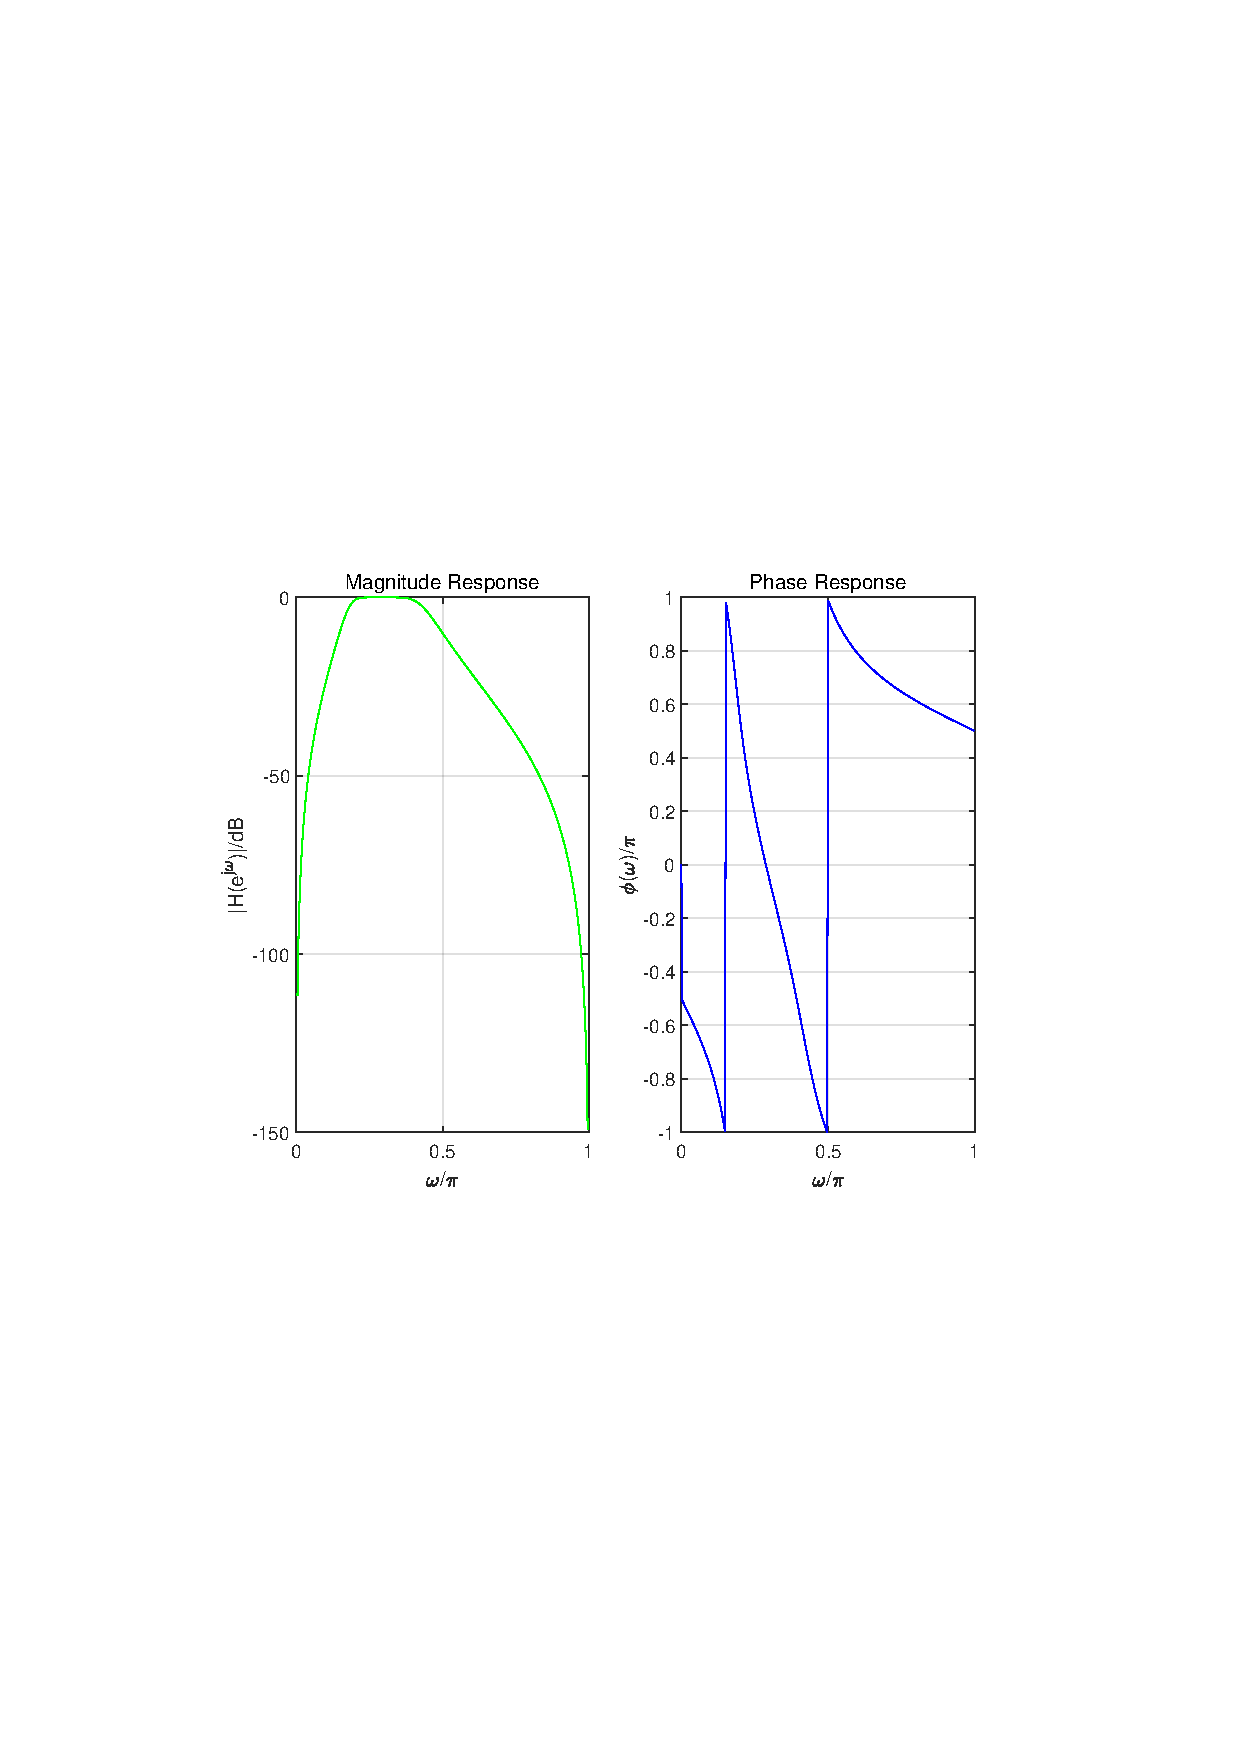
\includegraphics[width=14cm]{figure/BPBF.pdf}
	\caption{数字巴特沃斯带通滤波器频率响应曲线} \label{fig:BPBF}
\end{figure}

\subsubsection{带阻}

设置参数通带截止频率 Wp=[0.1,0.5],阻带截止频率 Ws=[0.2,0.4],通带最大衰减系数 Rp=1,阻带最小衰减系数 Rs=10。数字巴特沃斯带阻滤波器频率响应曲线如图 \ref{fig:BSBF} 所示。$\omega=0.2$ 时幅度为 -11.0dB,$\omega=0.4$ 时幅度为 -10.5dB,$\omega=0.1$ 时幅度为 0dB,$\omega=0.5$ 时幅度为 -0.7dB,通带满足指标要求,阻带满足指标要求,过渡带比指标要求的窄。

\begin{figure}[hbtp]
	\centering
	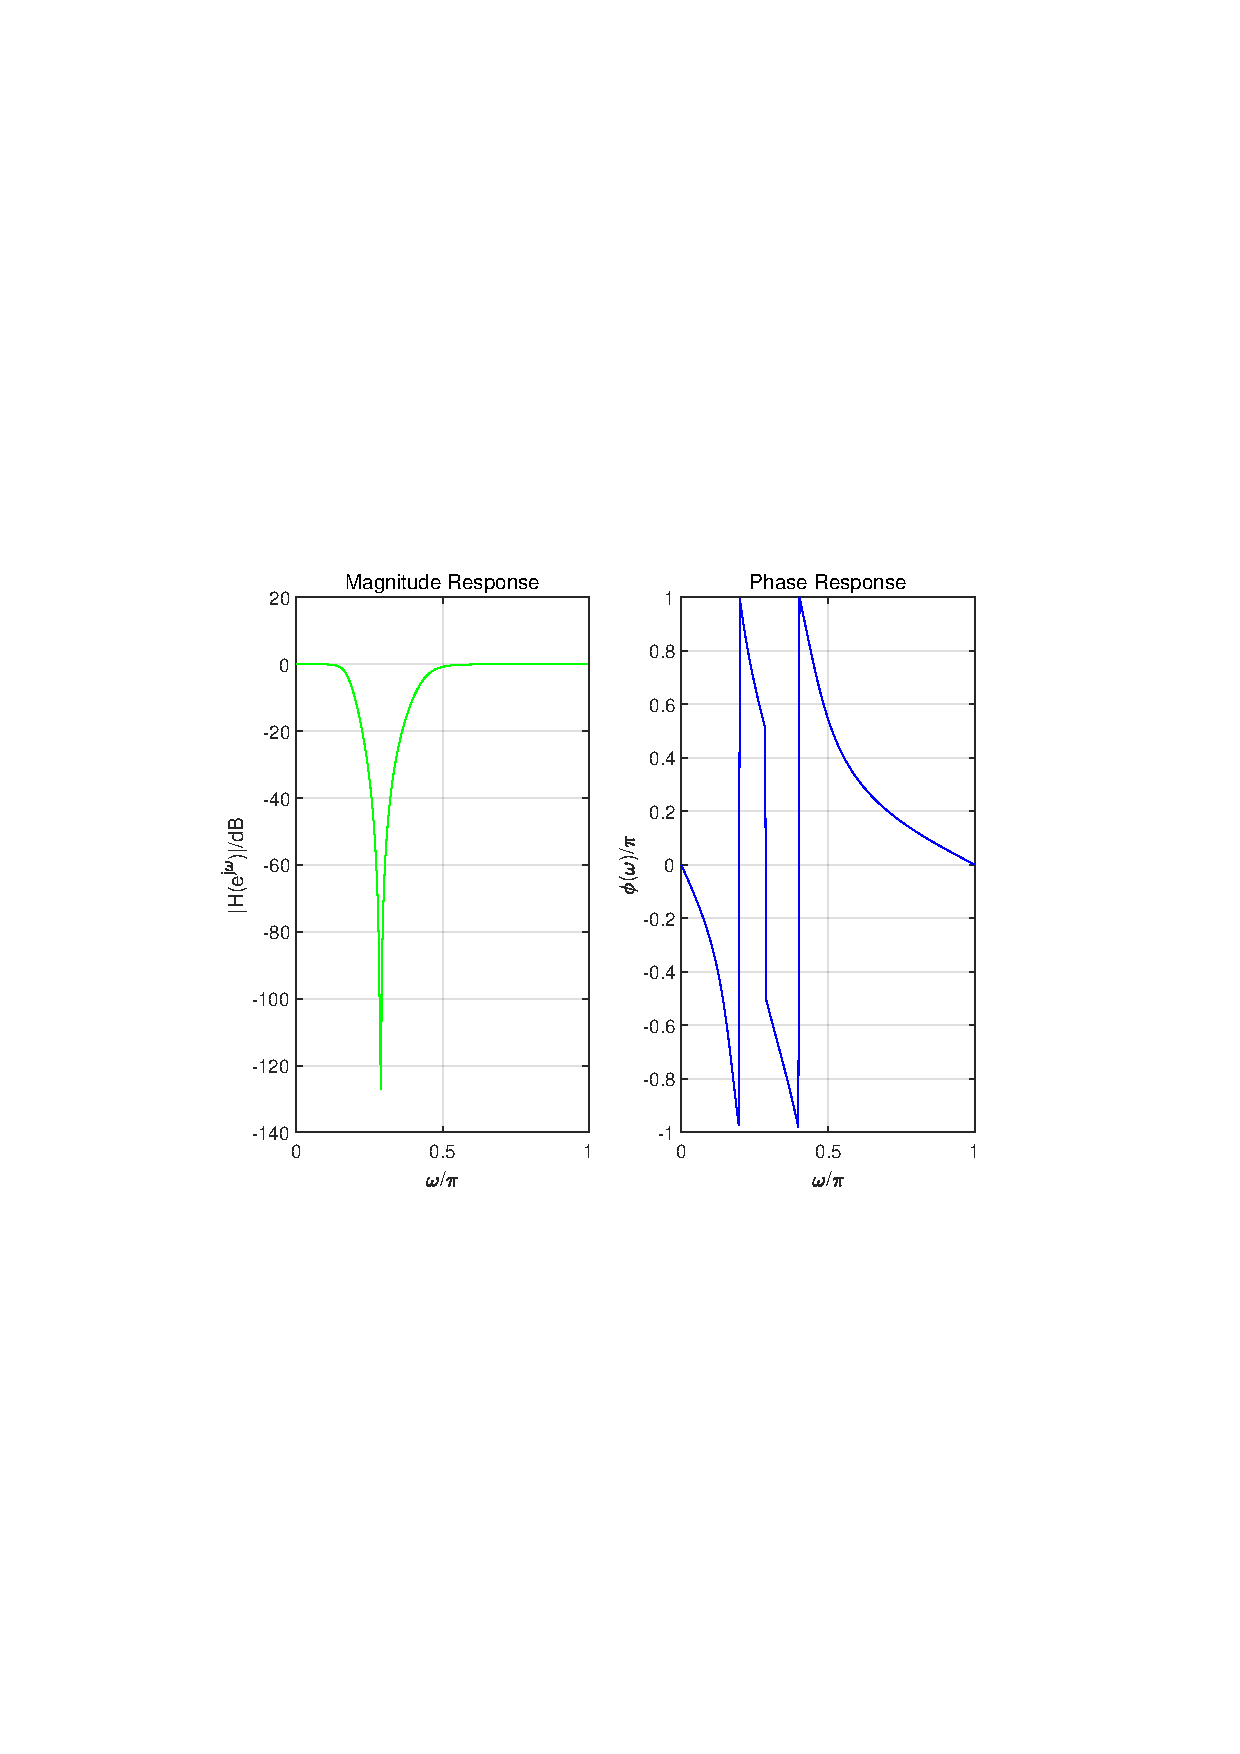
\includegraphics[width=14cm]{figure/BSBF.pdf}
	\caption{数字巴特沃斯带阻滤波器频率响应曲线} \label{fig:BSBF}
\end{figure}

\subsection{切比雪夫 I 型滤波器设计}

MATLAB 信号处理工具箱中提供了设计切比雪夫 I 型模拟滤波器的函数 cheb1ord、cheb1ap 和 cheby1,格式如下:

\begin{enumerate}[(1)]
\item \lstinline[language=Matlab]|[N,Wpo]=cheb1ord(Wp,Ws,Rp,Rs,'s');|
\item \lstinline[language=Matlab]|[z,p,G]=cheb1ap(N,Rp)|
\item \lstinline[language=Matlab]|[B,A]=cheby1(N,Rp,Wpo,'ftype','s');|
\end{enumerate}

其中,格式 (1) 和 (3) 中的 Wpo 是切比雪夫 I 型模拟低通滤波器的通带截止频率,而不是 3dB 截止频率,其他参数的含义与巴特沃斯滤波器设计函数中的参数相同。

\subsubsection{低通}

设置参数通带截止频率 Wp=0.2,阻带截止频率 Ws=0.4,通带最大衰减系数 Rp=1,阻带最小衰减系数 Rs=10。数字切比雪夫 I 型低通滤波器频率响应曲线如图 \ref{fig:LPC1F} 所示。$\omega=0.2$ 时幅度为 -1.0dB,$\omega=0.4$ 时幅度为 -13.8dB,通带满足指标要求,阻带满足指标要求,过渡带比指标要求的窄。

\begin{figure}[hbtp]
	\centering
	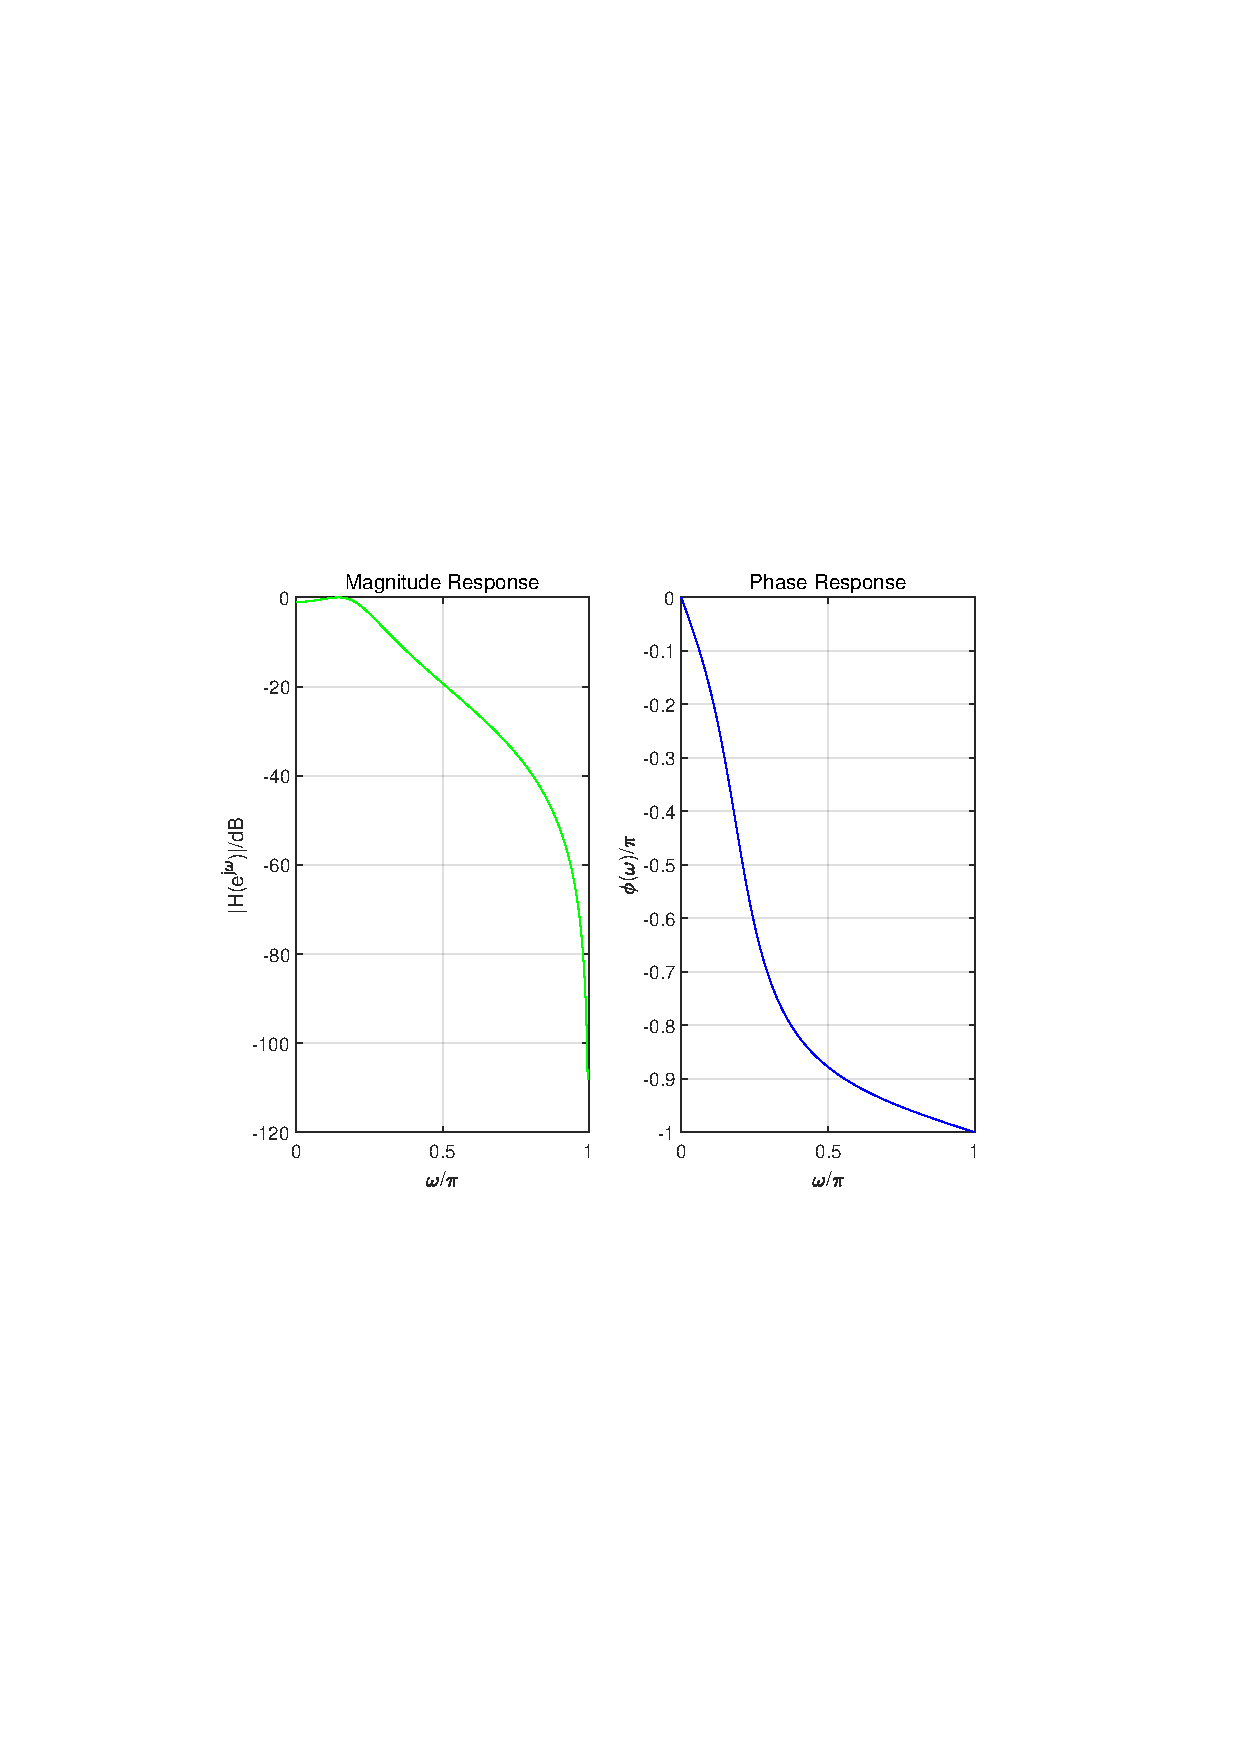
\includegraphics[width=14cm]{figure/LPC1F.pdf}
	\caption{数字切比雪夫 I 型低通滤波器频率响应曲线} \label{fig:LPC1F}
\end{figure}

\subsubsection{高通}

设置参数通带截止频率 Wp=0.4,阻带截止频率 Ws=0.2,通带最大衰减系数 Rp=1,阻带最小衰减系数 Rs=10。数字切比雪夫 I 型高通滤波器频率响应曲线如图 \ref{fig:HPC1F} 所示。$\omega=0.2$ 时幅度为 -13.5dB,$\omega=0.4$ 时幅度为 -1.0dB,通带满足指标要求,阻带满足指标要求,过渡带比指标要求的窄。

\begin{figure}[hbtp]
	\centering
	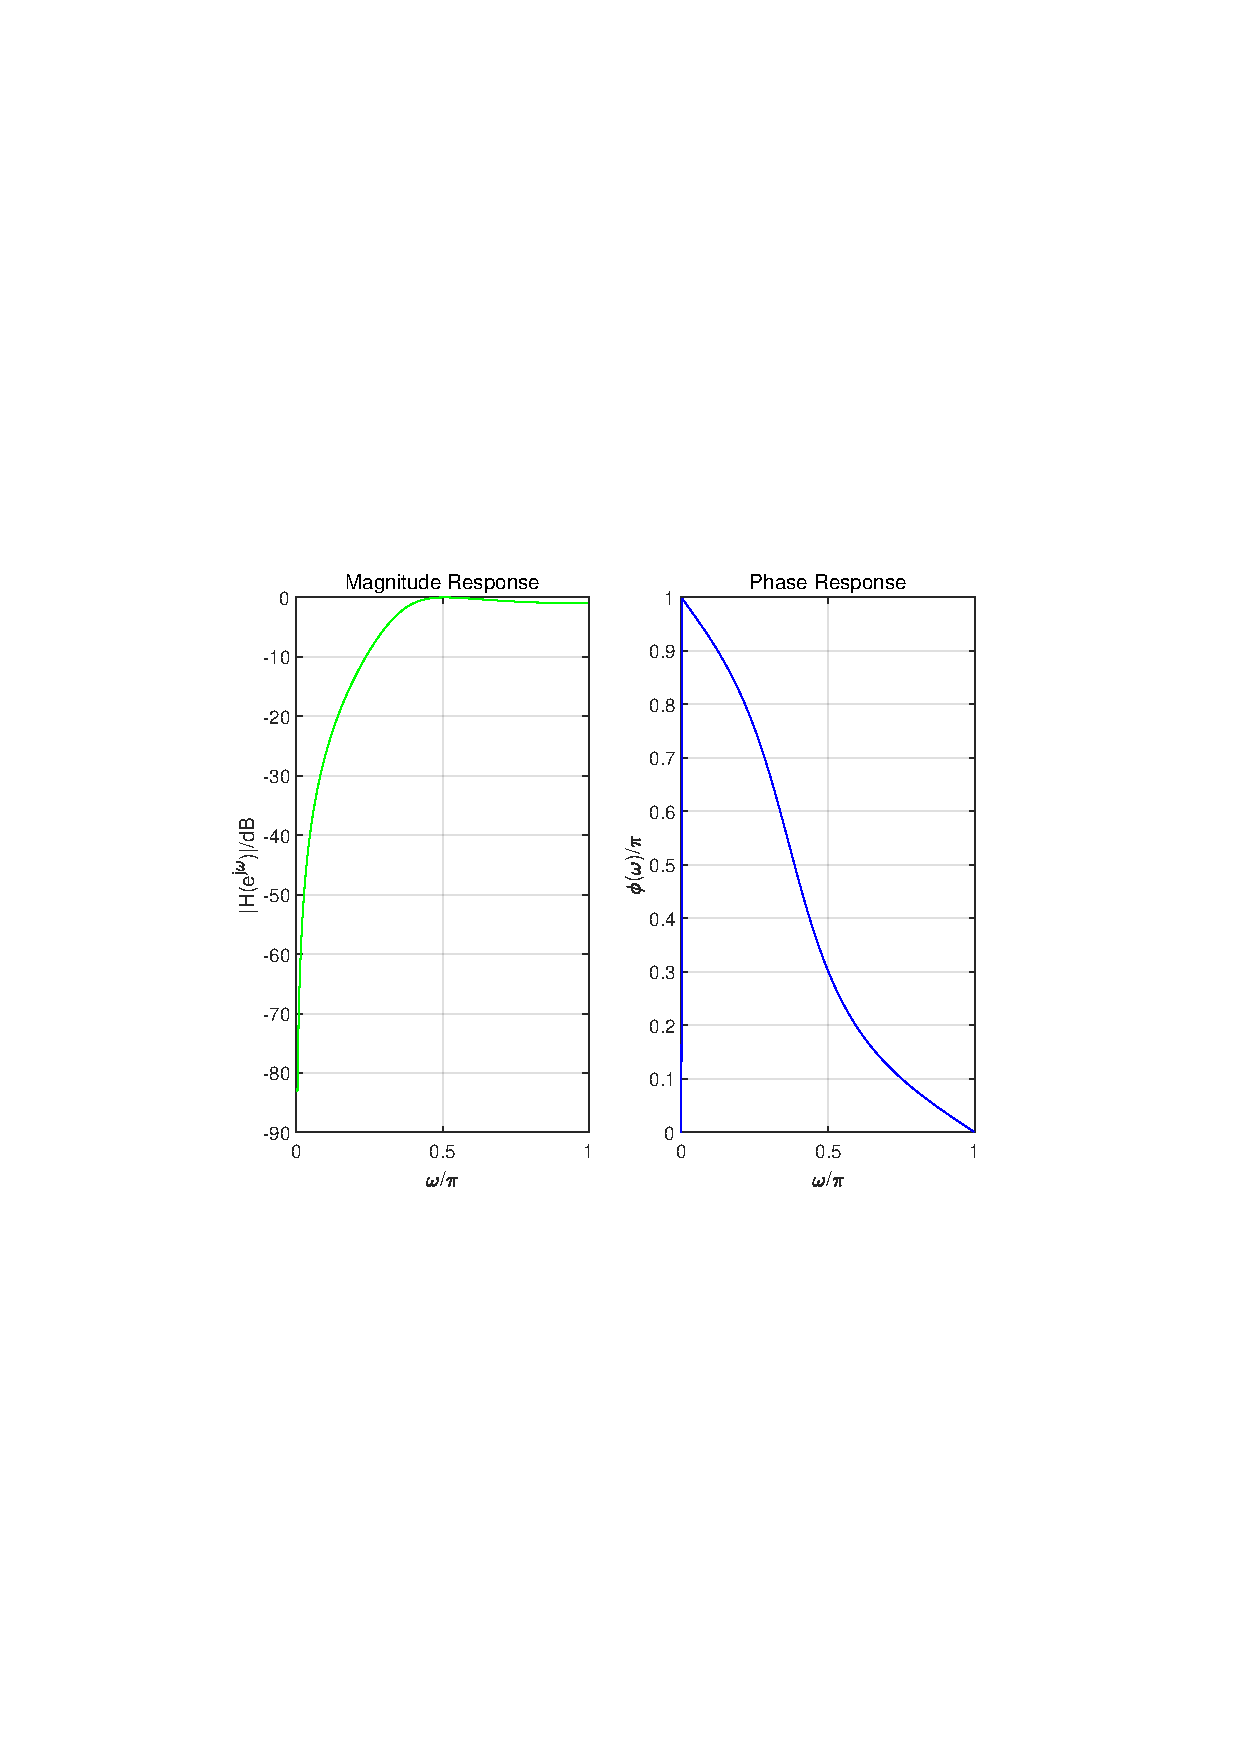
\includegraphics[width=14cm]{figure/HPC1F.pdf}
	\caption{数字切比雪夫 I 型高通滤波器频率响应曲线} \label{fig:HPC1F}
\end{figure}

\subsubsection{带通}

设置参数通带截止频率 Wp=[0.2,0.4],阻带截止频率 Ws=[0.1,0.5],通带最大衰减系数 Rp=1,阻带最小衰减系数 Rs=10。数字切比雪夫 I 型带通滤波器频率响应曲线如图 \ref{fig:BPC1F} 所示。$\omega=0.2$ 时幅度为 -1.0dB,$\omega=0.4$ 时幅度为 -1.1dB,$\omega=0.1$ 时幅度为 -20.2dB,$\omega=0.5$ 时幅度为 -10.4dB,通带略微不满足指标要求,阻带满足指标要求,过渡带比指标要求的窄。

\begin{figure}[hbtp]
	\centering
	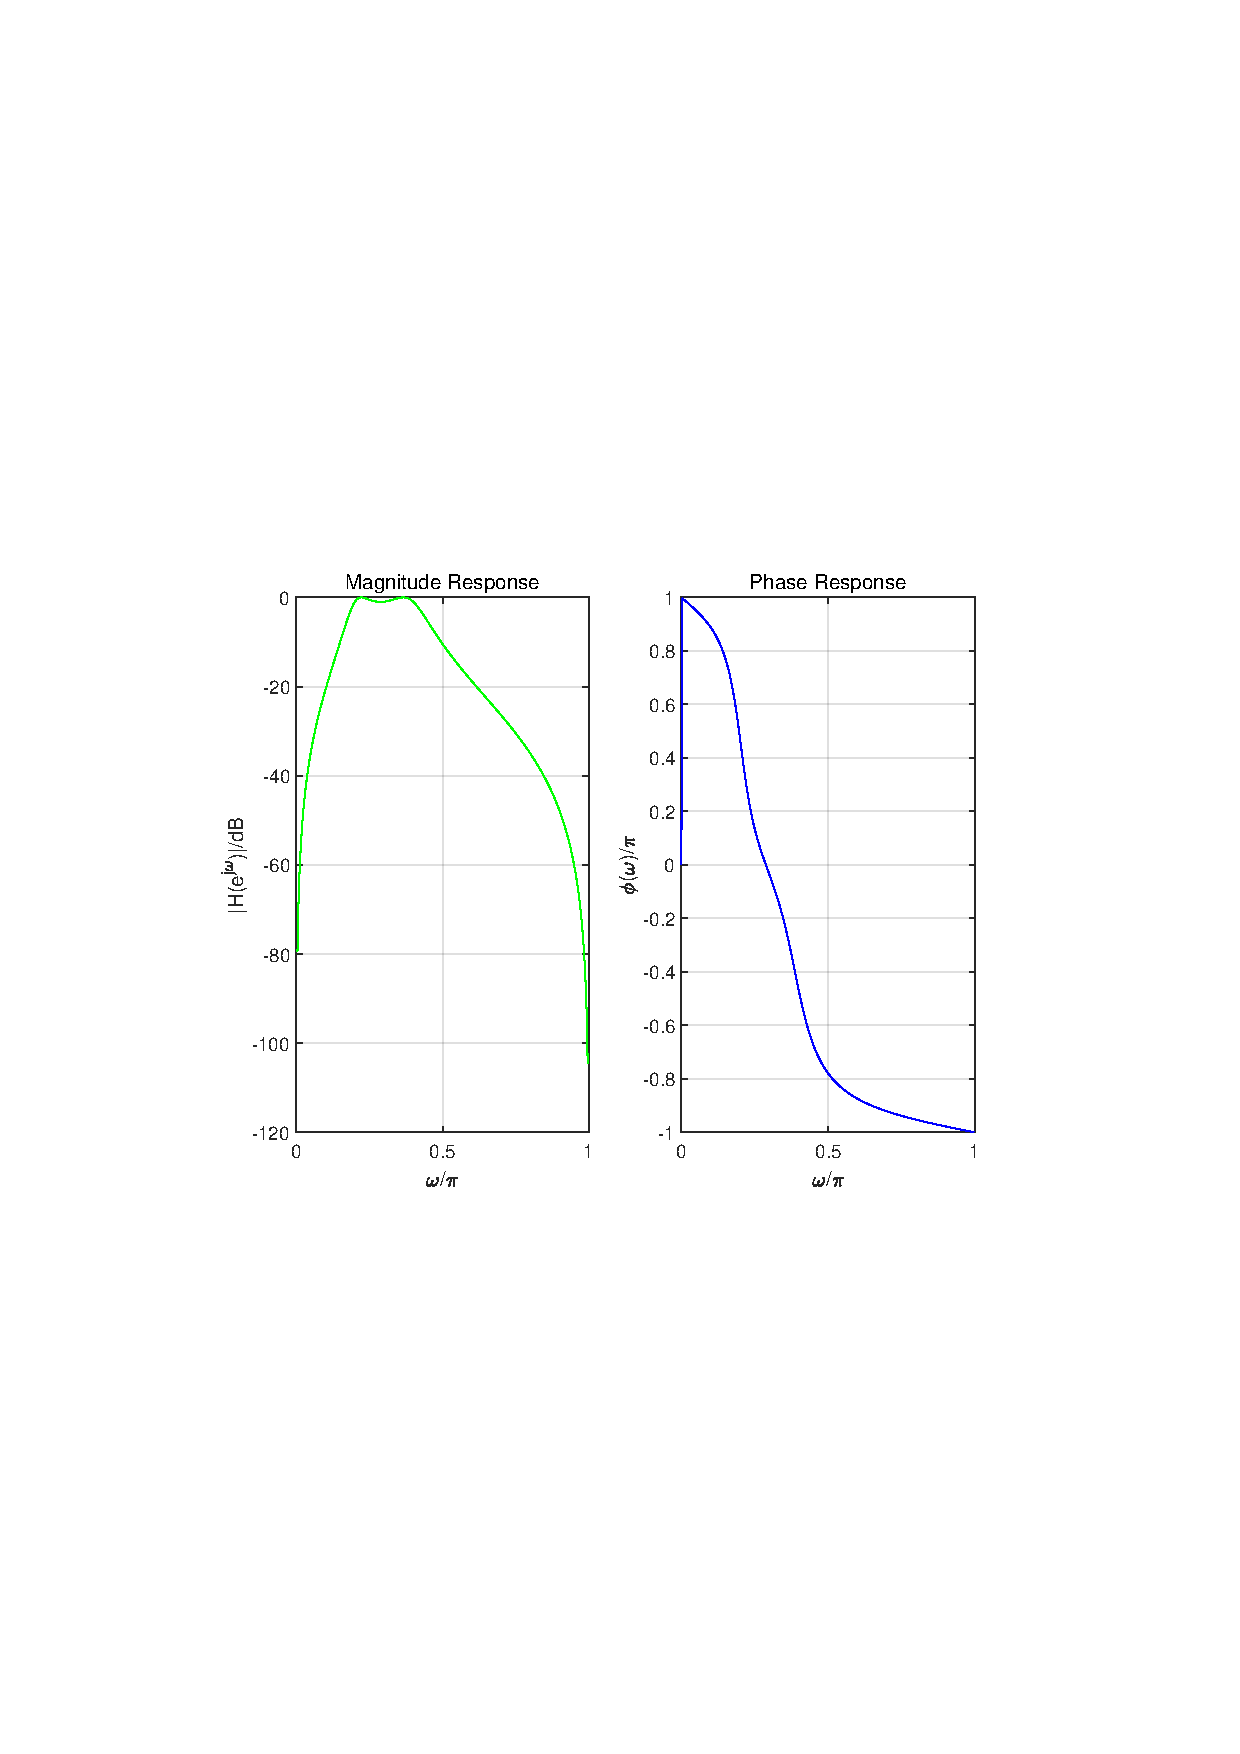
\includegraphics[width=14cm]{figure/BPC1F.pdf}
	\caption{数字切比雪夫 I 型带通滤波器频率响应曲线} \label{fig:BPC1F}
\end{figure}

\subsubsection{带阻}

设置参数通带截止频率 Wp=[0.1,0.5],阻带截止频率 Ws=[0.2,0.4],通带最大衰减系数 Rp=1,阻带最小衰减系数 Rs=10。数字切比雪夫 I 型带阻滤波器频率响应曲线如图 \ref{fig:BSC1F} 所示。$\omega=0.2$ 时幅度为 -28.2dB,$\omega=0.4$ 时幅度为 -7.6dB,$\omega=0.1$ 时幅度为 -1.1dB,$\omega=0.5$ 时幅度为 -1.0dB,通带略微不满足指标要求,阻带不满足指标要求,过渡带比指标要求一边窄一边宽。

\begin{figure}[hbtp]
	\centering
	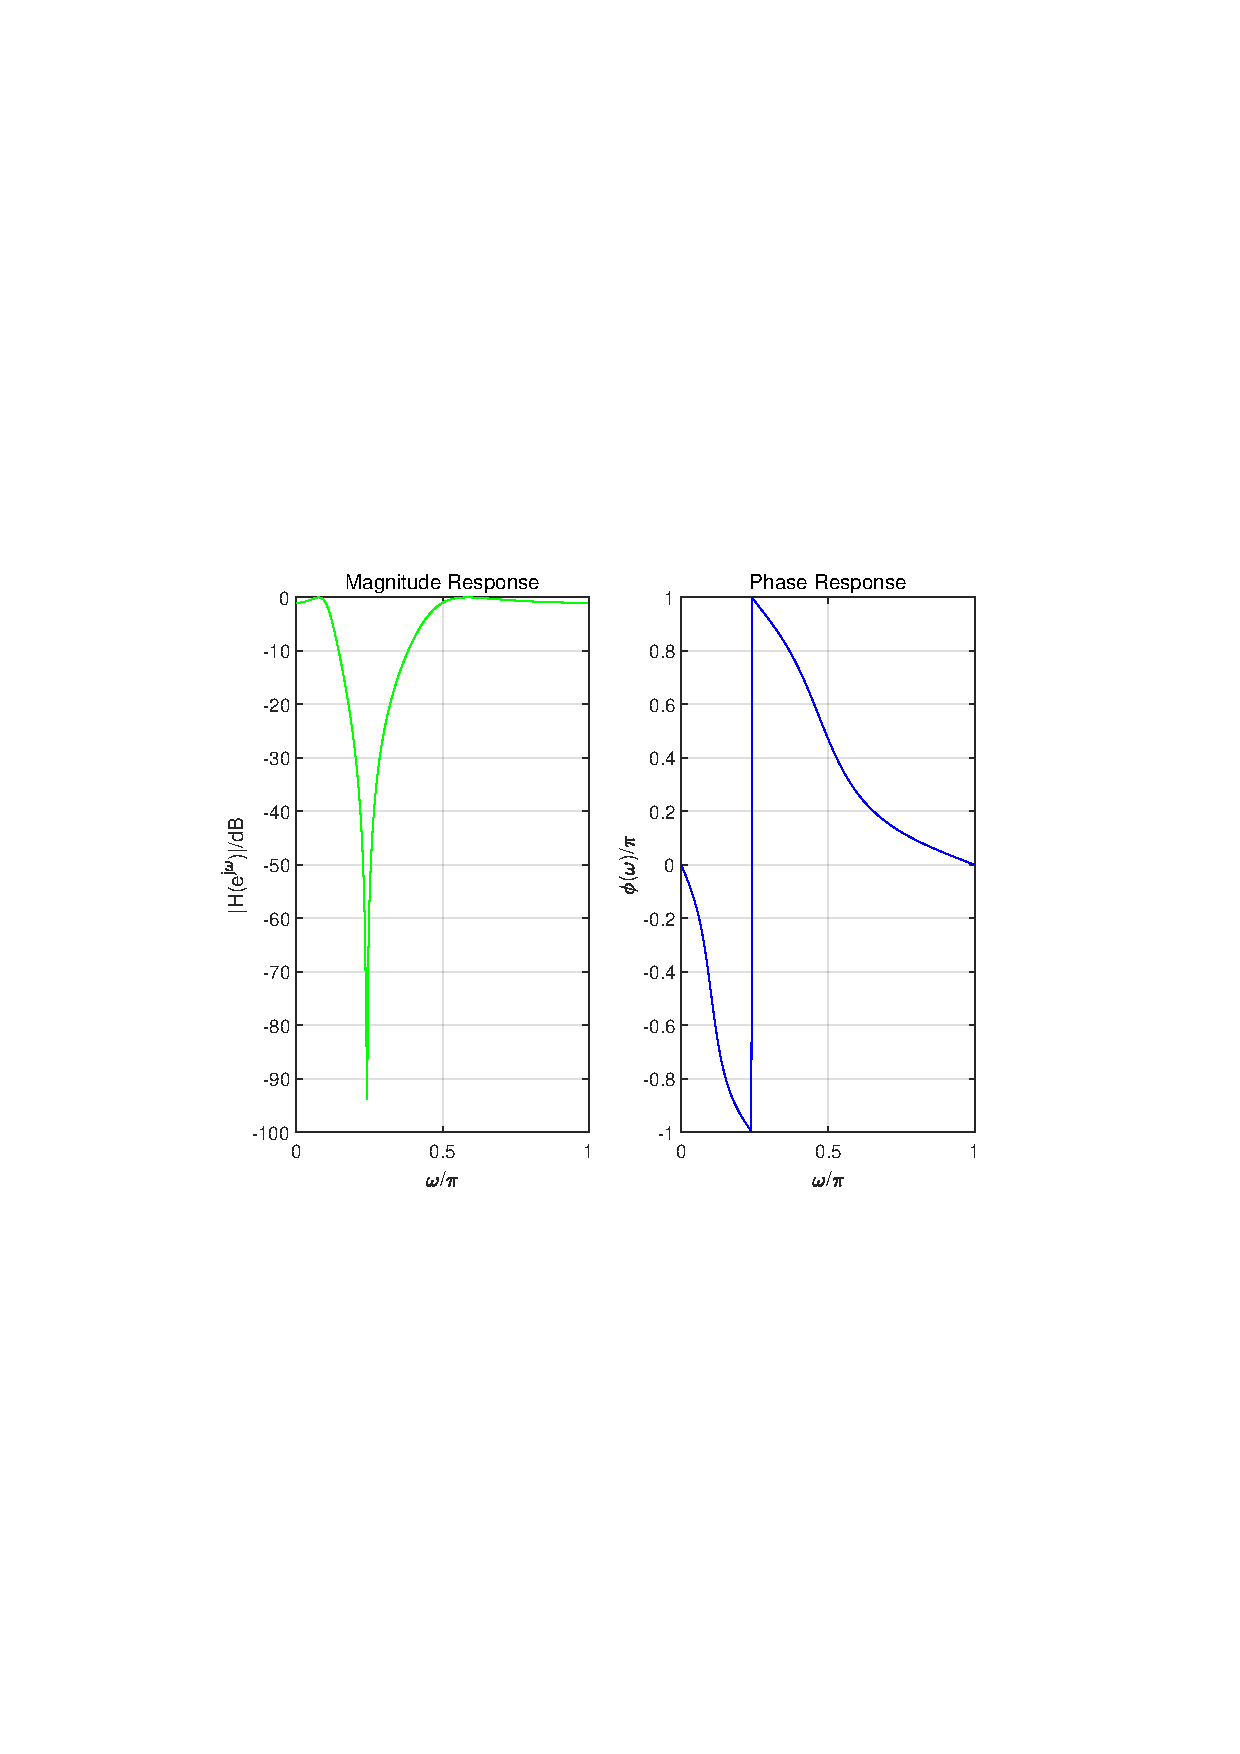
\includegraphics[width=14cm]{figure/BSC1F.pdf}
	\caption{数字切比雪夫 I 型带阻滤波器频率响应曲线} \label{fig:BSC1F}
\end{figure}

\subsection{切比雪夫 II 型滤波器设计}

MATLAB 信号处理工具箱中提供了设计切比雪夫 II 型模拟滤波器的函数 cheb2ord、cheb2ap 和 cheby2,格式如下:

\begin{enumerate}[(1)]
\item \lstinline[language=Matlab]|[N,Wso]=cheb2ord(Wp,Ws,Rp,Rs,'s');|
\item \lstinline[language=Matlab]|[z,p,G]=cheb2ap(N,Rs)|
\item \lstinline[language=Matlab]|[B,A]=cheby2(N,Rp,Wso,'ftype','s');|
\end{enumerate}

其中,格式 (1) 和 (3) 中的 Wso 是切比雪夫 II 型模拟低通滤波器的阻带截止频率,单位为 rad/s,其他参数的含义与巴特沃斯滤波器设计函数中的参数相同。

\subsubsection{低通}

设置参数通带截止频率 Wp=0.2,阻带截止频率 Ws=0.4,通带最大衰减系数 Rp=1,阻带最小衰减系数 Rs=10。数字切比雪夫 II 型低通滤波器频率响应曲线如图 \ref{fig:LPC2F} 所示。$\omega=0.2$ 时幅度为 0dB,$\omega=0.4$ 时幅度为 -1.1dB,通带满足指标要求,阻带不满足指标要求,过渡带比指标要求的宽。

\begin{figure}[hbtp]
	\centering
	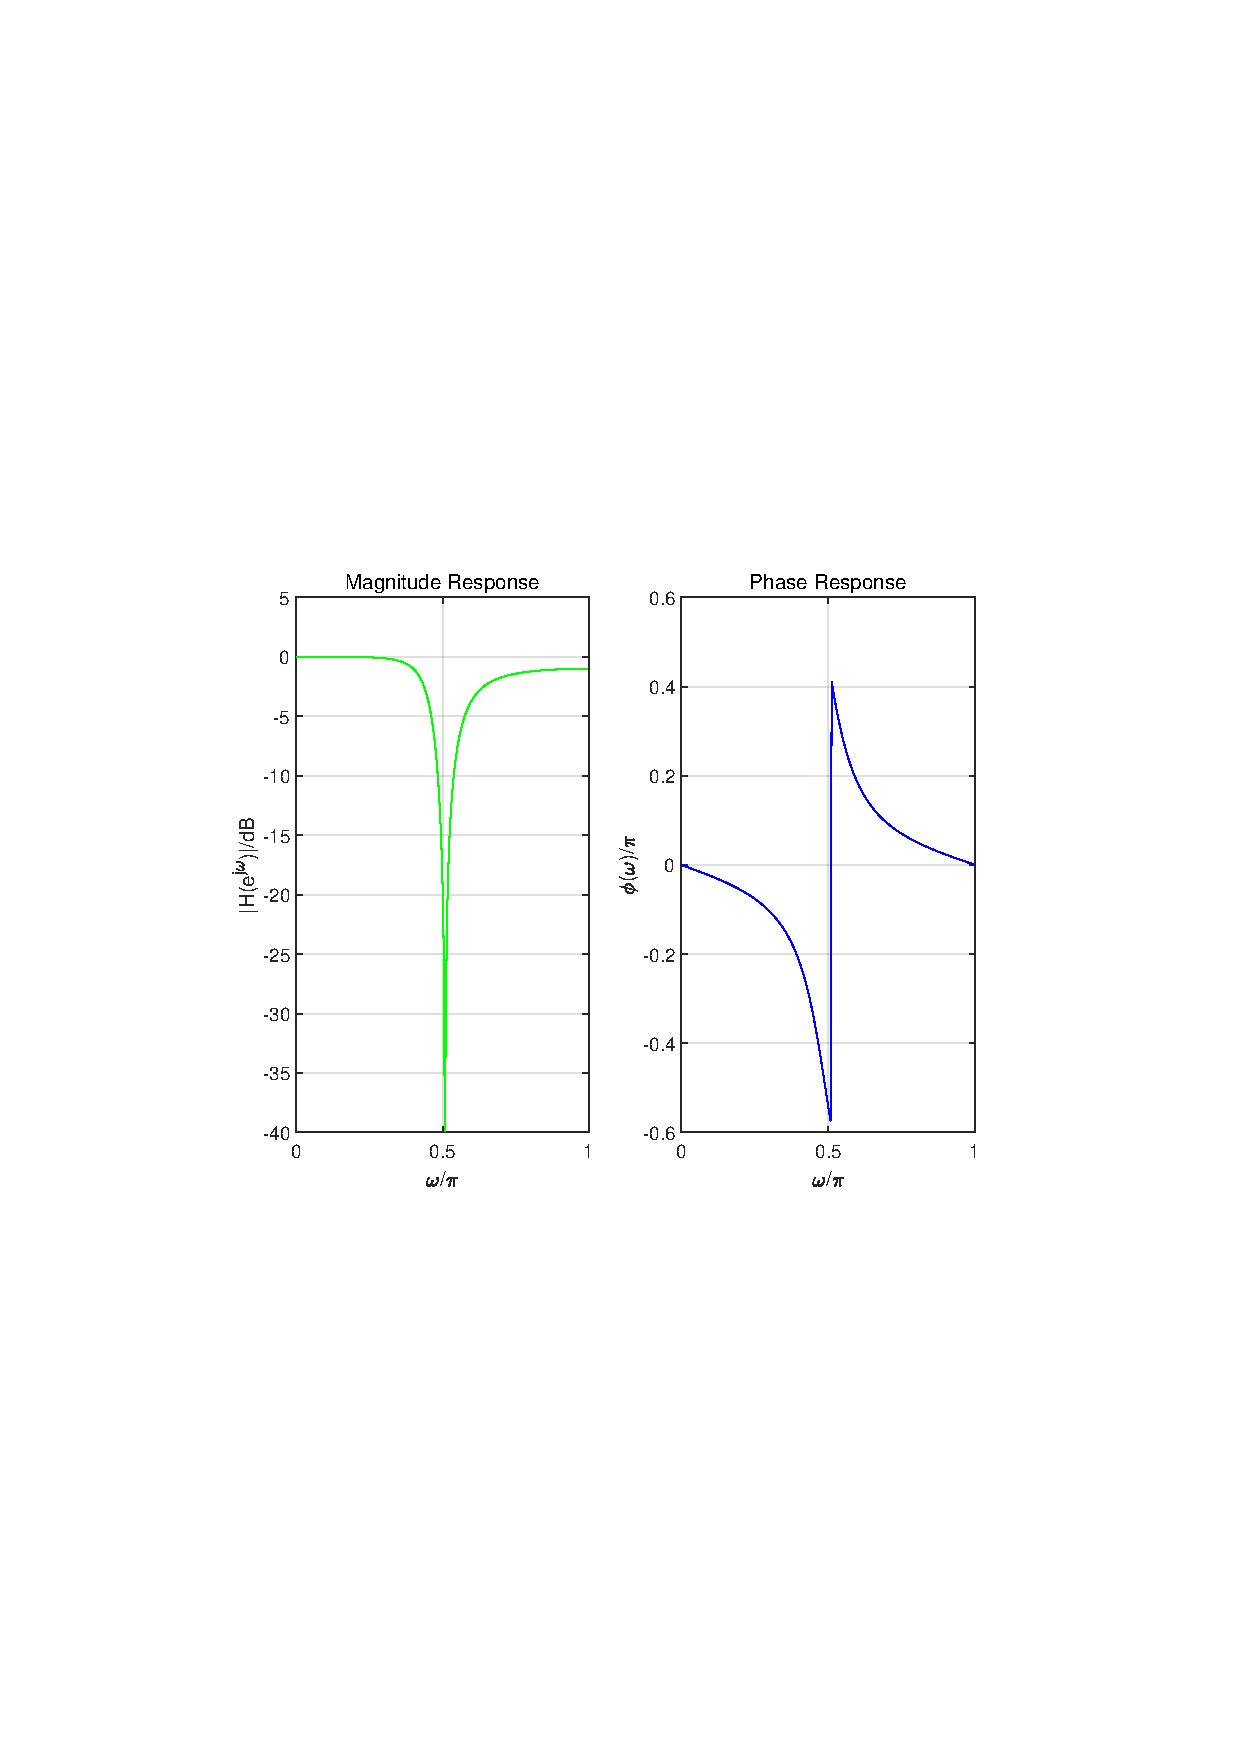
\includegraphics[width=14cm]{figure/LPC2F.pdf}
	\caption{数字切比雪夫 II 型低通滤波器频率响应曲线} \label{fig:LPC2F}
\end{figure}

\subsubsection{高通}

设置参数通带截止频率 Wp=0.4,阻带截止频率 Ws=0.2,通带最大衰减系数 Rp=1,阻带最小衰减系数 Rs=10。数字切比雪夫 II 型高通滤波器频率响应曲线如图 \ref{fig:HPC2F} 所示。$\omega=0.2$ 时幅度为 -0.9dB,$\omega=0.4$ 时幅度为 0dB,通带满足指标要求,阻带不满足指标要求,过渡带比指标要求的宽。

\begin{figure}[hbtp]
	\centering
	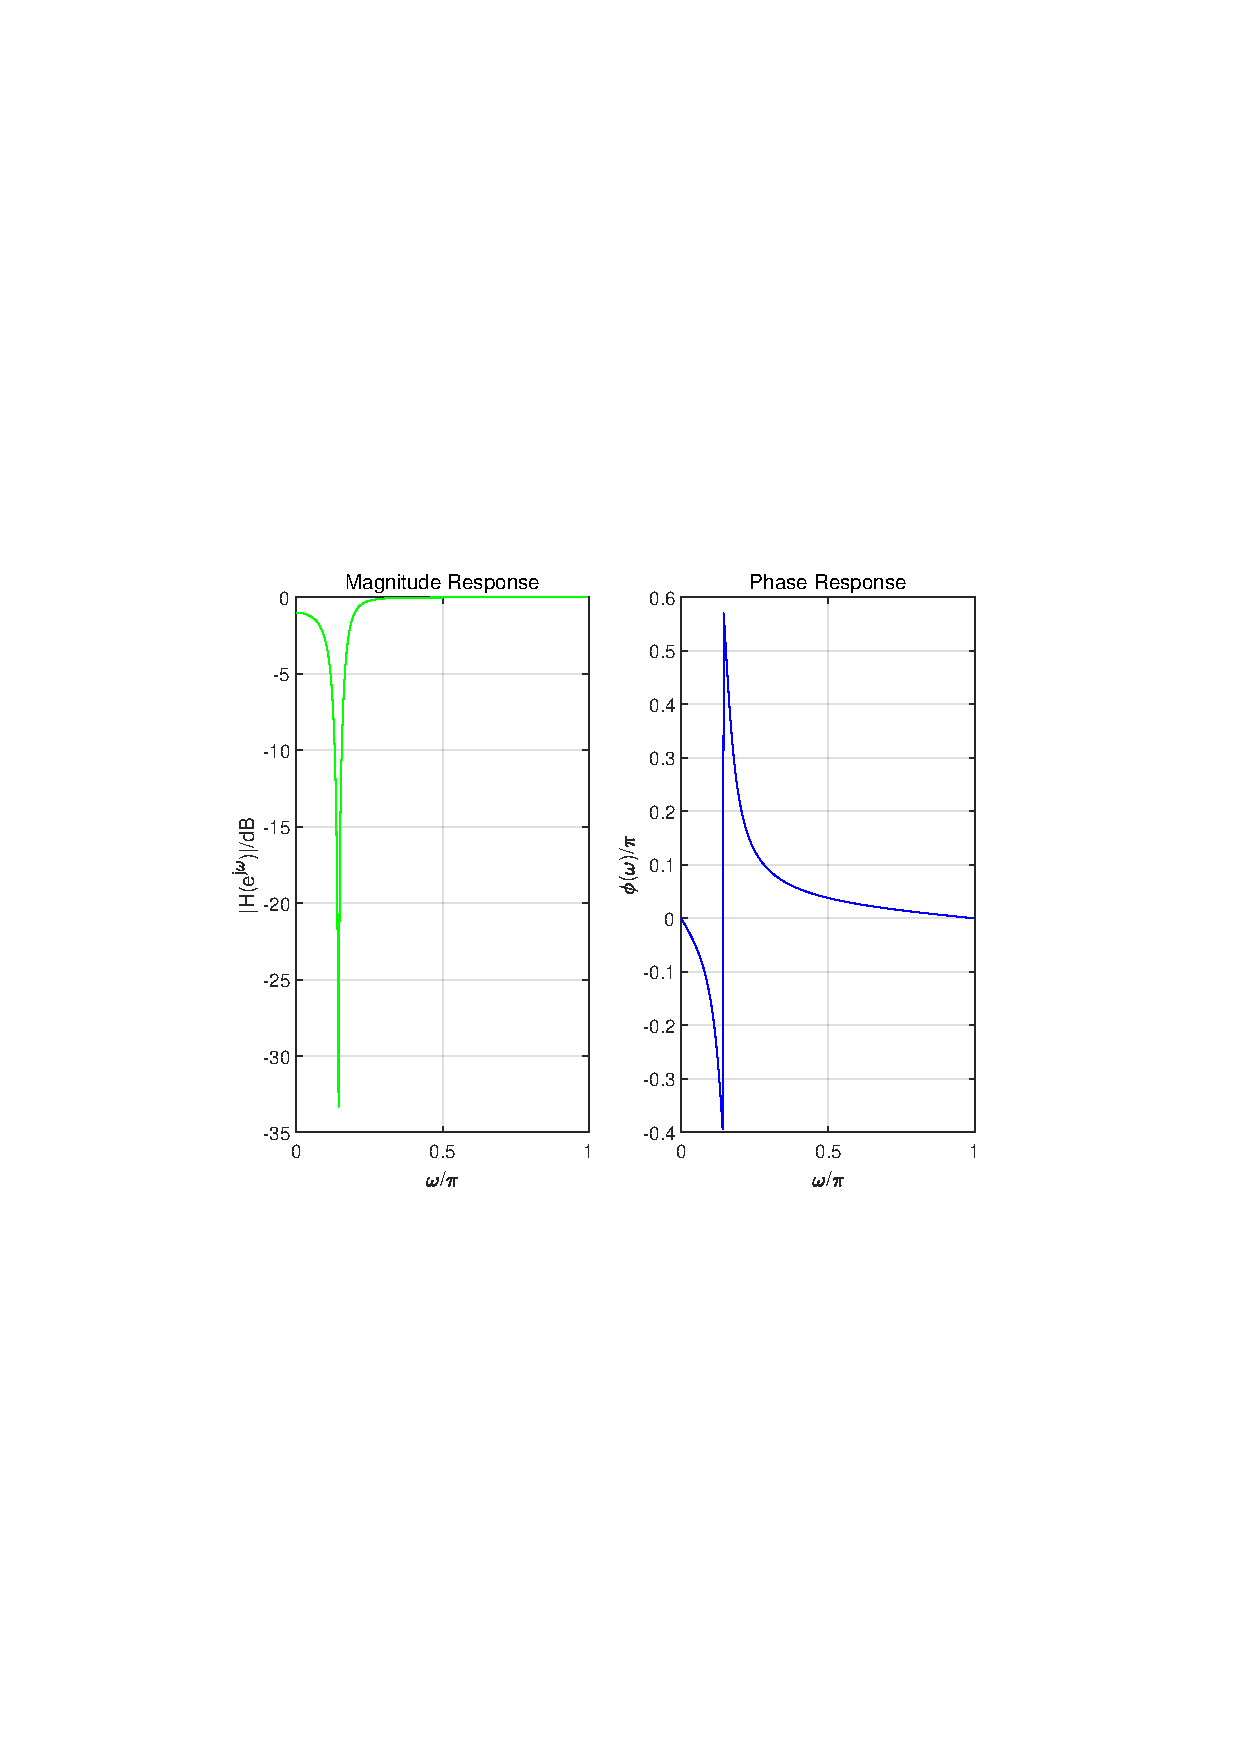
\includegraphics[width=14cm]{figure/HPC2F.pdf}
	\caption{数字切比雪夫 II 型高通滤波器频率响应曲线} \label{fig:HPC2F}
\end{figure}

\subsubsection{带通}

设置参数通带截止频率 Wp=[0.2,0.4],阻带截止频率 Ws=[0.1,0.5],通带最大衰减系数 Rp=1,阻带最小衰减系数 Rs=10。数字切比雪夫 II 型带通滤波器频率响应曲线如图 \ref{fig:BPC2F} 所示。$\omega=0.2$ 时幅度为 0dB,$\omega=0.4$ 时幅度为 0dB,$\omega=0.1$ 时幅度为 -0.9dB,$\omega=0.5$ 时幅度为 -1dB,通带满足指标要求,阻带不满足指标要求,过渡带比指标要求的宽。

\begin{figure}[hbtp]
	\centering
	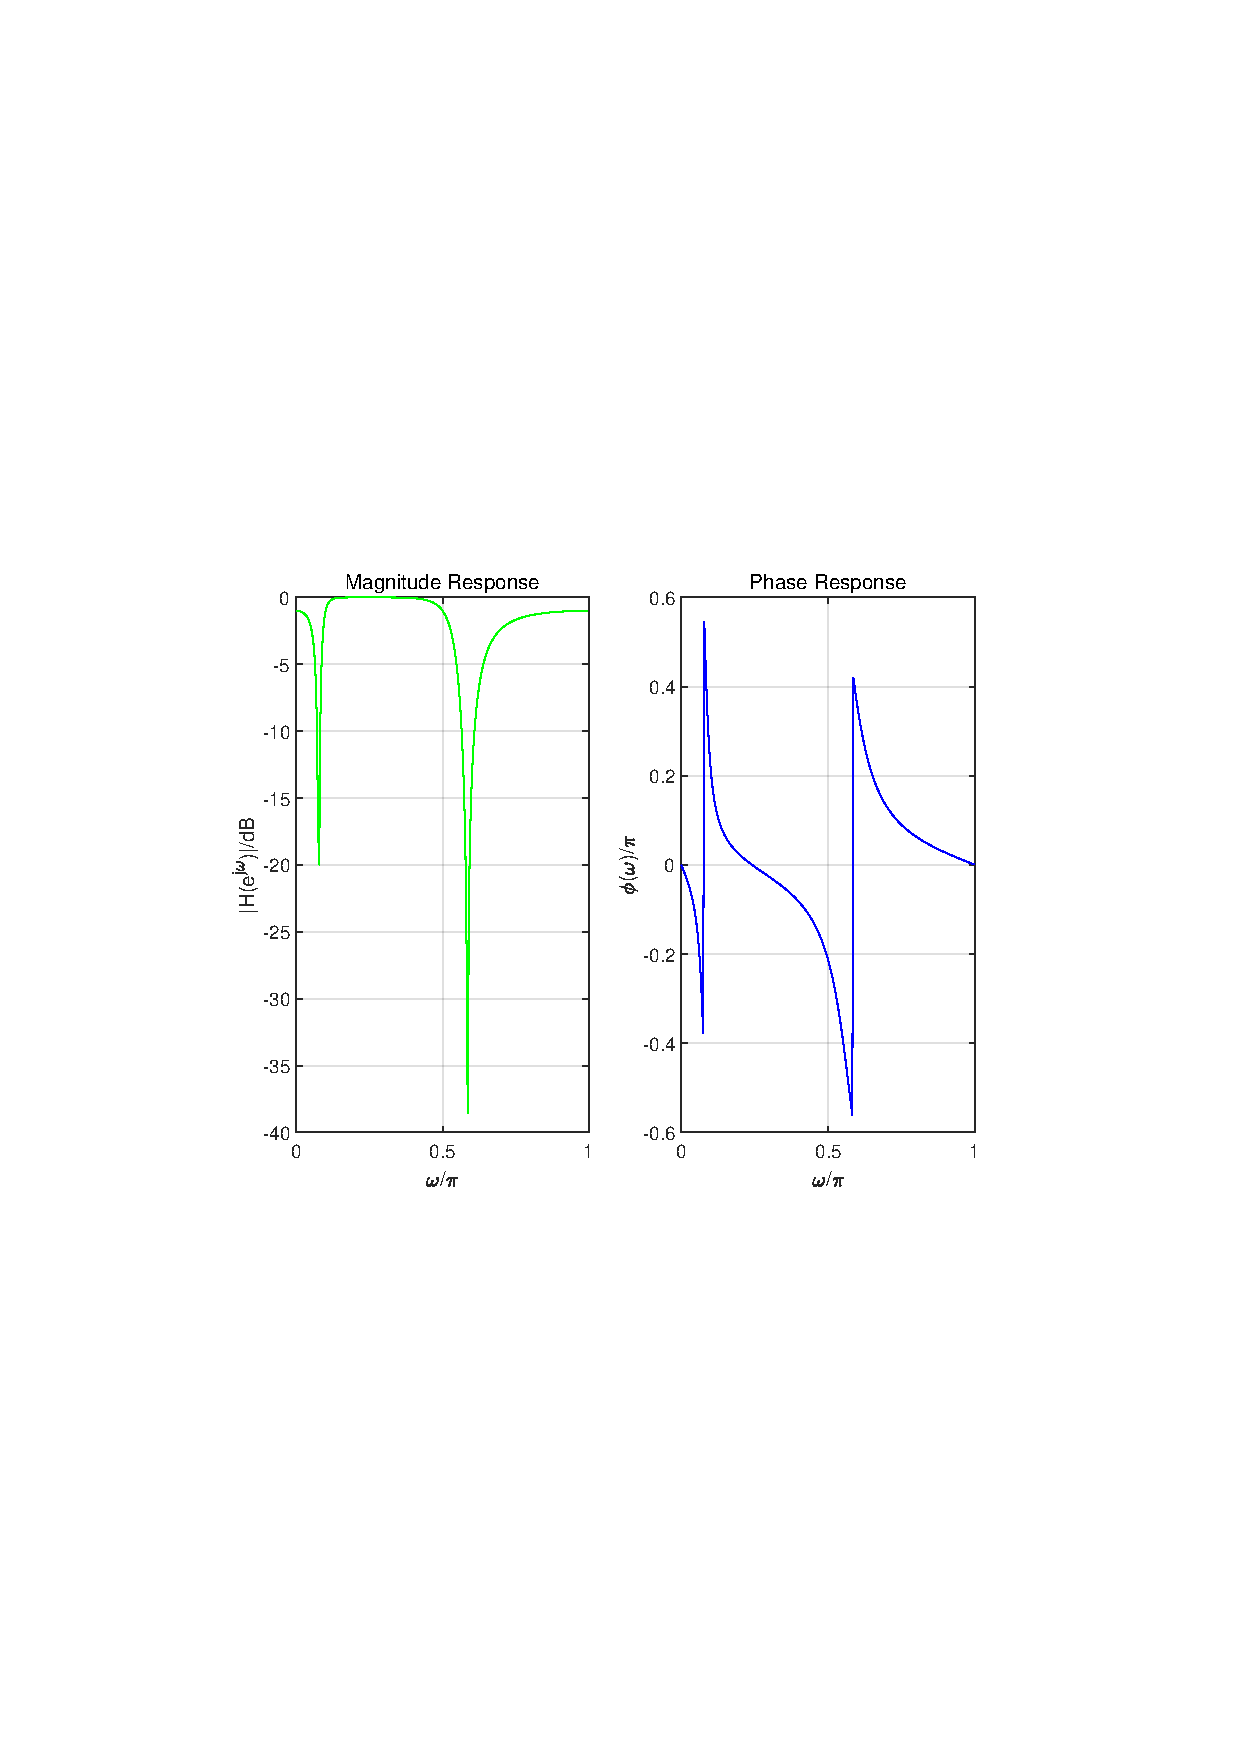
\includegraphics[width=14cm]{figure/BPC2F.pdf}
	\caption{数字切比雪夫 II 型带通滤波器频率响应曲线} \label{fig:BPC2F}
\end{figure}

\subsubsection{带阻}

设置参数通带截止频率 Wp=[0.1,0.5],阻带截止频率 Ws=[0.2,0.4],通带最大衰减系数 Rp=1,阻带最小衰减系数 Rs=10。数字切比雪夫 II 型带阻滤波器频率响应曲线如图 \ref{fig:BSC2F} 所示。$\omega=0.2$ 时幅度为 -1.0dB,$\omega=0.4$ 时幅度为 -0.9dB,$\omega=0.1$ 时幅度为 0dB,$\omega=0.5$ 时幅度为 0dB,通带满足指标要求,阻带不满足指标要求,过渡带比指标要求的宽。

\begin{figure}[hbtp]
	\centering
	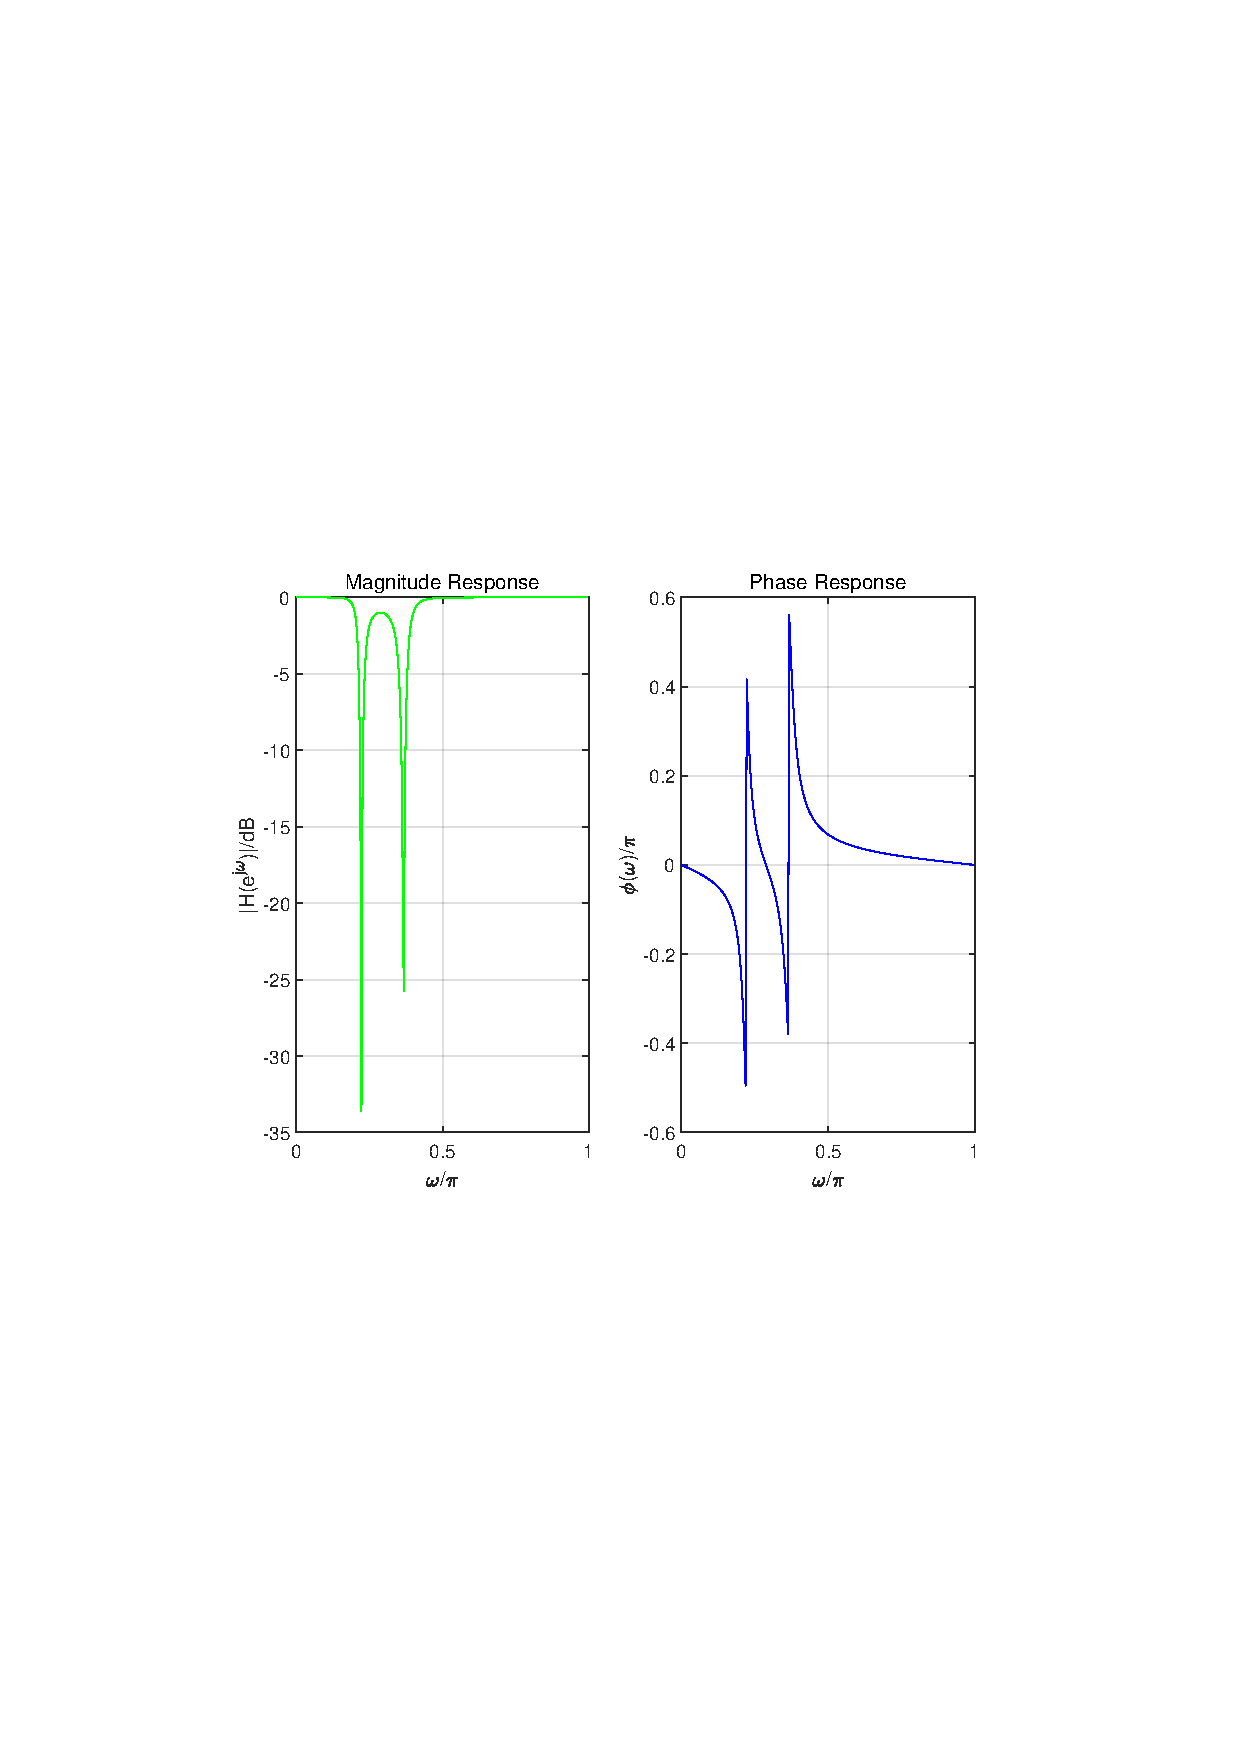
\includegraphics[width=14cm]{figure/BSC2F.pdf}
	\caption{数字切比雪夫 II 型带阻滤波器频率响应曲线} \label{fig:BSC2F}
\end{figure}

\subsection{IIR 数字滤波器的信号流图}


假设系统函数为
%
\begin{equation}
H(z)=\frac{Y(z)}{X(z)}=\frac{\displaystyle\sum_{k=0}^Mb_kz^{-k}}{1-\displaystyle\sum_{k=1}^Na_kz^{-k}}=H_1(z)H_2(z)
\end{equation}
%
其中
%
\begin{align}
H_1(z) &= \sum_{k=0}^Mb_kz^{-k} \\
H_2(z) &= \frac{1}{1-\displaystyle\sum_{k=1}^Na_kz^{-k}}
\end{align}
%
IIR 数字滤波器的直接 I 型结构如图 \ref{fig:direct1} 所示,直接 II 型结构如图 \ref{fig:direct2} 所示。

\begin{figure}[htbp]
	\centering
	\begin{minipage}[t]{0.48\textwidth}
		\centering
		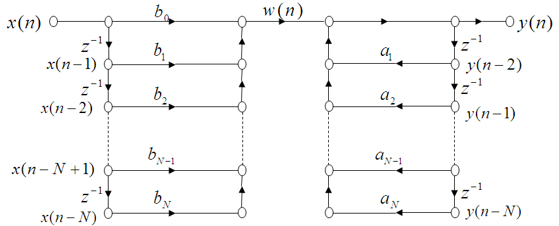
\includegraphics[width=6cm]{figure/direct1.png}
		\caption{直接 I 型} \label{fig:direct1}
	\end{minipage}
	\begin{minipage}[t]{0.48\textwidth}
		\centering
		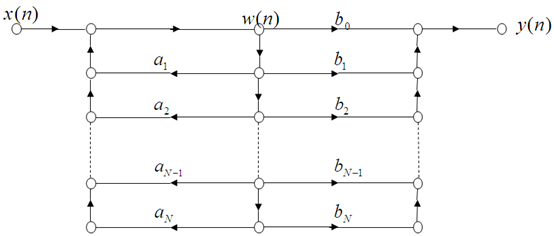
\includegraphics[width=6cm]{figure/direct2.png}
		\caption{直接 II 型} \label{fig:direct2}
	\end{minipage}
\end{figure}


假设系统函数为:
%
\begin{equation}
H(z)=A\prod_{k=1}^{L}\frac{1+\beta_{1k}z^{-1}+\beta_{2k}z^{-2}}{1-\alpha_{1k}z^{-1}-\alpha_{2k}}=A\prod_{k=1}^LH_k(z)
\end{equation}
%
其中 $H_k(z)$ 称为滤波器的二阶基本节。系统可用 $L$ 个二阶子系统的级联构成,如图 \ref{fig:cascade} 所示。

\begin{figure}[hbtp]
	\centering
	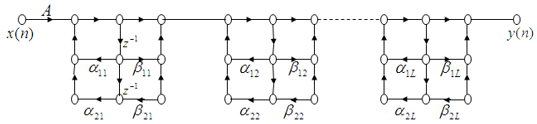
\includegraphics[width=16cm]{figure/cascade.png}
	\caption{IIR 数字滤波器的级联结构} \label{fig:cascade}
\end{figure}

假设系统函数为:
%
\begin{equation}
H(z)=C+\sum_{k=1}^L\frac{\gamma_{0k}+\gamma_{1k}z^{-1}}{1+\beta_{1k}z^{-1}+\beta_{2k}z^{-2}}=C+\sum_{k=1}^LH_k(z)
\end{equation}
%
其中 $H_k(z)$ 是二阶子系统,整个滤波器由常增益支路与 $L$ 个二阶子系统并联构成,每个子系统均采用直接 II 型结构,如图 \ref{fig:parallel} 所示。

\begin{figure}[hbtp]
	\centering
	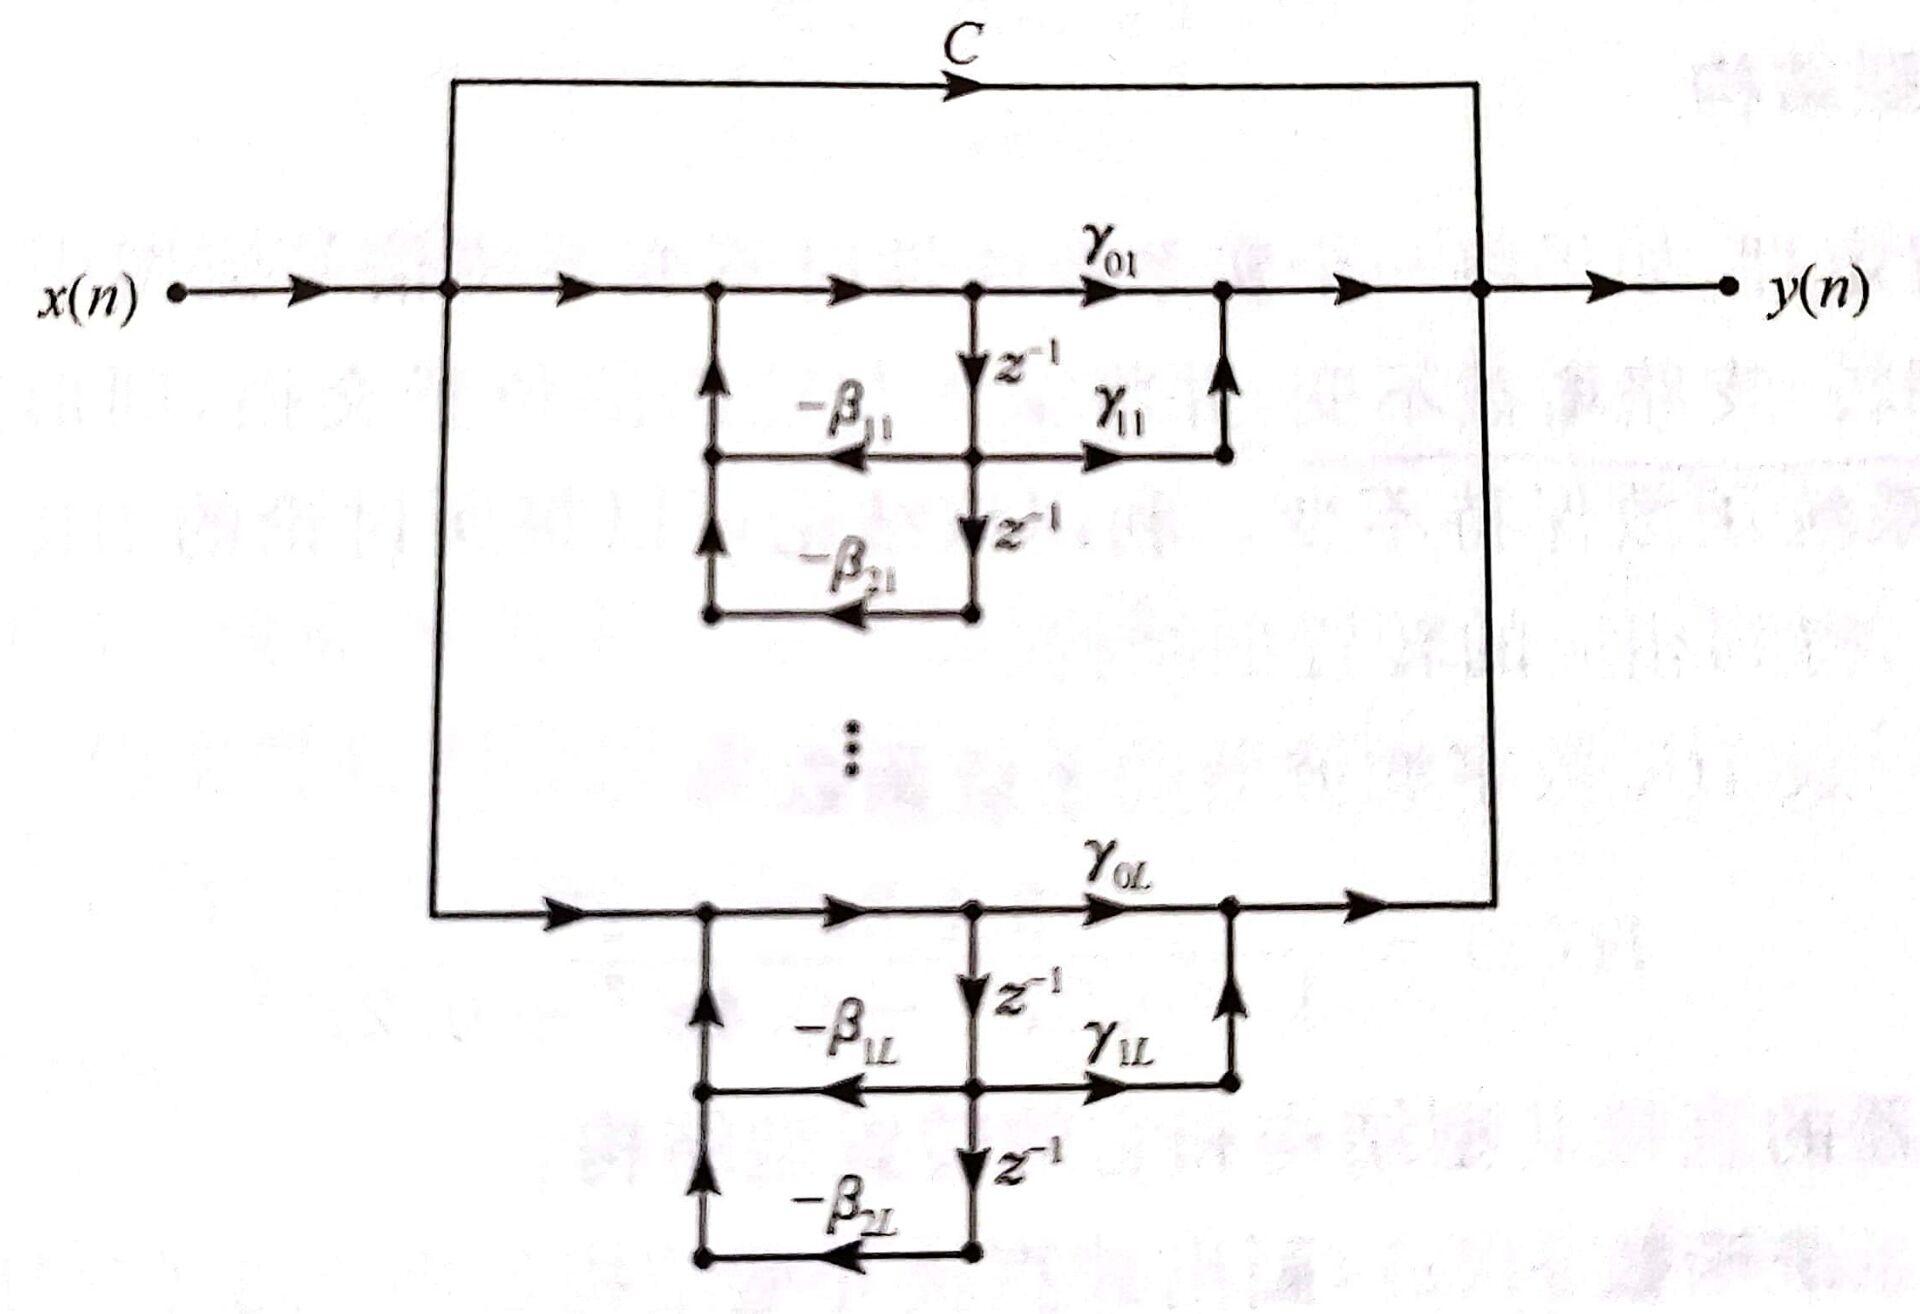
\includegraphics[width=8cm]{figure/parallel.jpg}
	\caption{IIR 数字滤波器的并联联结构} \label{fig:parallel}
\end{figure}

\section{总结}

\subsection{杨文韬}

\begin{itemize}
\item 问题1:从实验结果比较这些滤波器的区别?

\begin{enumerate}[1.]
\item \textbf{巴特沃斯滤波器}的频率特性曲线,无论在通带内还是阻带内都是频率的单调函数。因此,当通带的边界处满足指标要求时,通带内肯定会有裕量。所以,更有效的设计方法应该是将精确度均匀的分布在整个通带或阻带内,或者同时分布在两者之内。这样就可用较低阶数的系统满足要求。这可通过选择具有等波纹特性的逼近函数来达到。
\item \textbf{切比雪夫 I 型滤波器}幅度特性在通带内是等波纹的,在阻带内是单调下降的。\textbf{切比雪夫 II 型滤波器}幅度特性在通带内是单调的,在阻带内是等波纹的。切比雪夫 I 型滤波器在阻带跟通带过渡时要比切比雪夫 II 型滤波器过渡时平稳许多,所以切比雪夫 I 型滤波器要比切比雪夫 II 型滤波器所做出来的效果要好。
\end{enumerate}

\item 问题2:Python 中是否有类似的设计滤波器函数?

scipy.signal 库中有类似函数,\lstinline[language=Python]|scipy.signal.buttord(wp, ws, gpass, gstop, analog=False, fs=None)|、\lstinline[language=Python]|scipy.signal.cheb1ord(wp, ws, gpass, gstop, analog=False, fs=None)| 和 \lstinline[language=Python]|scipy.signal.cheb2ord(wp, ws, gpass, gstop, analog=False, fs=None)|。wp 和 ws 指通带和阻带频率;gpass 指通带中的最大损耗 (dB);gstop 指阻带中的最小衰减(dB);analog 为可选参数,如果为True,则返回一个模拟滤波器,否则返回一个数字滤波器;fs 为可选参数,数字系统的采样频率。
\end{itemize}

\subsection{刘浩}

\begin{itemize}
\item 问题:IIR 数字滤波器信号流图各有什么特点?

\begin{itemize}
\item \textbf{直接 I 型}:先实现系统函数的零点,再实现极点;需要 2N 个延迟器和 2N 个乘法器。
\item \textbf{直接 II 型}:先实性系统函数的极点,再实现零点;需要 N 个延迟器和 2N 个乘法器。
\item \textbf{级联型}:(1) 二阶基本节搭配灵活,可调换次序;(2) 可直接控制零极点;(3) 存储器最少;(4) 误差较大。
\item \textbf{并联型}:(1) 可单独调整极点,不能直接控制零点;(2) 误差小,各基本节的误差不相互影响;(3) 速度快。
\end{itemize}
\end{itemize}

\subsection{周泽熙}

\begin{itemize}
\item 问题:在使用相关函数是如何正确理解参数?

例如 \lstinline[language=Matlab]|[N,Wc]=buttord(Wp,Ws,Rp,Rs)|,其中 Wp 和 Ws 分别是通带截止频率和阻带截止频率关于 $\pi$ 的归一化,所以切记 Wp 和 Ws 均属于$[0,1]$。Rp 和 Rs 则由公式 ( \ref{eq:1} ) 和 ( \ref{eq:2} ) 得到。在 \lstinline[language=Matlab]|[B,A]=butter(N,Wc,’ftype’)| 中,应注意ftype。ftpye=high,设计高通滤波器,ftype=stop,设计带阻滤波器。

\end{itemize}

% % 参考文献,此处以 MLA 引用格式为例

%\begin{thebibliography}{9}
%\end{thebibliography}

% % \includepdf[pages={1,2}]{Memo.pdf} 

% 可以直接导入pdf页面
\newpage
\begin{appendices}  % 附录环境
\section{实验代码}

\subsection{巴特沃斯滤波器设计}

\begin{lstlisting}[language=Matlab]
%低通
Wp=0.2;Ws=0.4;Rp=1;Rs=10;
[N,Wc]=buttord(Wp,Ws,Rp,Rs);
[B,A]=butter(N,Wc);
[H,w]=freqz(B,A,256);
subplot(1,2,1);
plot(w/pi,20*log10(abs(H)),'g');grid on;
xlabel('\omega/\pi');
ylabel('|H(e^j^\omega)|/dB');
title('Magnitude Response');
subplot(1,2,2);
plot(w/pi,angle(H)/pi,'b');grid on;
xlabel('\omega/\pi');
ylabel('\phi(\omega)/\pi');
title('Phase Response');
\end{lstlisting}

\begin{lstlisting}[language=Matlab]
%高通
Wp=0.4;Ws=0.2;Rp=1;Rs=10;
[N,Wc]=buttord(Wp,Ws,Rp,Rs);
[B,A]=butter(N,Wc,'high');
[H,w]=freqz(B,A,256);
subplot(1,2,1);
plot(w/pi,20*log10(abs(H)));grid on;
xlabel('\omega/\pi');
ylabel('|H(e^j^\omega)|/dB');
title('Magnitude Response');
subplot(1,2,2);
plot(w/pi,angle(H)/pi);grid on;
xlabel('\omega/\pi');
ylabel('\phi(\omega)/\pi');
title('Phase Response');
\end{lstlisting}

\begin{lstlisting}[language=Matlab]
%带通
Wp=[0.1,0.5];Ws=[0.2,0.4];Rp=1;Rs=10;
[N,Wc]=buttord(Wp,Ws,Rp,Rs);
[B,A]=butter(N,Wc);
[H,w]=freqz(B,A,256);
subplot(1,2,1);
plot(w/pi,20*log10(abs(H)),'g');grid on;
xlabel('\omega/\pi');
ylabel('|H(e^j^\omega)|/dB');
title('Magnitude Response');
subplot(1,2,2);
plot(w/pi,angle(H)/pi,'b');grid on;
xlabel('\omega/\pi');
ylabel('\phi(\omega)/\pi');
title('Phase Response');
\end{lstlisting}

\begin{lstlisting}[language=Matlab]
%带阻
Wp=[0.1,0.5];Ws=[0.2,0.4];Rp=1;Rs=10;
[N,Wc]=buttord(Wp,Ws,Rp,Rs);
[B,A]=butter(N,Wc,'stop');
[H,w]=freqz(B,A,256);
subplot(1,2,1);
plot(w/pi,20*log10(abs(H)),'g');grid on;
xlabel('\omega/\pi');
ylabel('|H(e^j^\omega)|/dB');
title('Magnitude Response');
subplot(1,2,2);
plot(w/pi,angle(H)/pi,'b');grid on;
xlabel('\omega/\pi');
ylabel('\phi(\omega)/\pi');
title('Phase Response');
\end{lstlisting}

\subsection{切比雪夫 I 型滤波器设计}

\begin{lstlisting}[language=Matlab]
%低通
Wp=0.2;Ws=0.4;Rp=1;Rs=10;
[N,Wpo]=cheb1ord(Wp,Ws,Rp,Rs);
[B,A]=cheby1(N,Rp,Wpo);
[H,w]=freqz(B,A,256);
subplot(1,2,1);
plot(w/pi,20*log10(abs(H)),'g');grid on;
xlabel('\omega/\pi');
ylabel('|H(e^j^\omega)|/dB');
title('Magnitude Response');
subplot(1,2,2);
plot(w/pi,angle(H)/pi,'b');grid on;
xlabel('\omega/\pi');
ylabel('\phi(\omega)/\pi');
title('Phase Response');
\end{lstlisting}

\begin{lstlisting}[language=Matlab]
%高通
Wp=0.4;Ws=0.2;Rp=1;Rs=10;
[N,Wpo]=cheb1ord(Wp,Ws,Rp,Rs);
[B,A]=cheby1(N,Rp,Wpo,'high');
[H,w]=freqz(B,A,256);
subplot(1,2,1);
plot(w/pi,20*log10(abs(H)),'g');grid on;
xlabel('\omega/\pi');
ylabel('|H(e^j^\omega)|/dB');
title('Magnitude Response');
subplot(1,2,2);
plot(w/pi,angle(H)/pi,'b');grid on;
xlabel('\omega/\pi');
ylabel('\phi(\omega)/\pi');
title('Phase Response');
\end{lstlisting}

\begin{lstlisting}[language=Matlab]
%带通
Wp=[0.2,0.4];Ws=[0.1,0.5];Rp=1;Rs=10;
[N,Wpo]=cheb1ord(Wp,Ws,Rp,Rs);
[B,A]=cheby1(N,Rp,Wpo);
[H,w]=freqz(B,A,256);
subplot(1,2,1);
plot(w/pi,20*log10(abs(H)),'g');grid on;
xlabel('\omega/\pi');
ylabel('|H(e^j^\omega)|/dB');
title('Magnitude Response');
subplot(1,2,2);
plot(w/pi,angle(H)/pi,'b');grid on;
xlabel('\omega/\pi');
ylabel('\phi(\omega)/\pi');
title('Phase Response');
\end{lstlisting}

\begin{lstlisting}[language=Matlab]
%带阻
Wp=[0.1,0.5];Ws=[0.2,0.4];Rp=1;Rs=10;
[N,Wpo]=cheb1ord(Wp,Ws,Rp,Rs);
[B,A]=cheby1(N,Rp,Wpo,'stop');
[H,w]=freqz(B,A,256);
subplot(1,2,1);
plot(w/pi,20*log10(abs(H)),'g');grid on;
xlabel('\omega/\pi');
ylabel('|H(e^j^\omega)|/dB');
title('Magnitude Response');
subplot(1,2,2);
plot(w/pi,angle(H)/pi,'b');grid on;
xlabel('\omega/\pi');
ylabel('\phi(\omega)/\pi');
title('Phase Response');
\end{lstlisting}

\subsection{切比雪夫 II 型滤波器设计}

\begin{lstlisting}[language=Matlab]
%低通
Wp=0.2;Ws=0.4;Rp=1;Rs=10;
[N,Wso]=cheb2ord(Wp,Ws,Rp,Rs);
[B,A]=cheby2(N,Rp,Wso);
[H,w]=freqz(B,A,256);
subplot(1,2,1);
plot(w/pi,20*log10(abs(H)),'g');grid on;
xlabel('\omega/\pi');
ylabel('|H(e^j^\omega)|/dB');
title('Magnitude Response');
subplot(1,2,2);
plot(w/pi,angle(H)/pi,'b');grid on;
xlabel('\omega/\pi');
ylabel('\phi(\omega)/\pi');
title('Phase Response');
\end{lstlisting}

\begin{lstlisting}[language=Matlab]
%高通
Wp=0.4;Ws=0.2;Rp=1;Rs=10;
[N,Wso]=cheb2ord(Wp,Ws,Rp,Rs);
[B,A]=cheby2(N,Rp,Wso,'high');
[H,w]=freqz(B,A,256);
subplot(1,2,1);
plot(w/pi,20*log10(abs(H)),'g');grid on;
xlabel('\omega/\pi');
ylabel('|H(e^j^\omega)|/dB');
title('Magnitude Response');
subplot(1,2,2);
plot(w/pi,angle(H)/pi,'b');grid on;
xlabel('\omega/\pi');
ylabel('\phi(\omega)/\pi');
title('Phase Response');
\end{lstlisting}

\begin{lstlisting}[language=Matlab]
%带通
Wp=[0.2,0.4];Ws=[0.1,0.5];Rp=1;Rs=10;
[N,Wso]=cheb2ord(Wp,Ws,Rp,Rs);
[B,A]=cheby2(N,Rp,Wso);
[H,w]=freqz(B,A,256);
subplot(1,2,1);
plot(w/pi,20*log10(abs(H)),'g');grid on;
xlabel('\omega/\pi');
ylabel('|H(e^j^\omega)|/dB');
title('Magnitude Response');
subplot(1,2,2);
plot(w/pi,angle(H)/pi,'b');grid on;
xlabel('\omega/\pi');
ylabel('\phi(\omega)/\pi');
title('Phase Response');
\end{lstlisting}

\begin{lstlisting}[language=Matlab]
%带阻
Wp=[0.1,0.5];Ws=[0.2,0.4];Rp=1;Rs=10;
[N,Wso]=cheb2ord(Wp,Ws,Rp,Rs);
[B,A]=cheby2(N,Rp,Wso,'stop');
[H,w]=freqz(B,A,256);
subplot(1,2,1);
plot(w/pi,20*log10(abs(H)),'g');grid on;
xlabel('\omega/\pi');
ylabel('|H(e^j^\omega)|/dB');
title('Magnitude Response');
subplot(1,2,2);
plot(w/pi,angle(H)/pi,'b');grid on;
xlabel('\omega/\pi');
ylabel('\phi(\omega)/\pi');
title('Phase Response');
\end{lstlisting}

%\section{核心层}\label{subsec:B}
\end{appendices}

\end{document}  % 结束